\documentclass[a4paper, 12pt]{article}

\usepackage[T2A]{fontenc}
\usepackage[utf8]{inputenc}
\usepackage[russian]{babel}
\usepackage{graphicx}
\usepackage[normalem]{ulem}
\graphicspath{{img/}}
\DeclareGraphicsExtensions{.pdf,.png,.jpg}

\usepackage[left=3cm, right=1cm, top=2cm, bottom=2cm, bindingoffset=0cm]{geometry}

\usepackage{setspace}
\usepackage{pdflscape}
% \usepackage[nodisplayskipstretch]{setspace}

\usepackage{longtable}
\linespread{1.3}
\usepackage{indentfirst}
\setlength{\parindent}{1.25cm}
\usepackage{mathtools}

\usepackage{caption}
\DeclareCaptionLabelFormat{gostfigure}{Рисунок #2}
\captionsetup*[figure]{labelformat=gostfigure}

\usepackage{hyperref}
\usepackage{xcolor}

\usepackage{color}
\usepackage{listings} %% собственно, это и есть пакет listings
\definecolor{darkgreen}{rgb}{0,0.5,0}

\sloppy

\definecolor{linkcolor}{HTML}{000000} % цвет ссылок
\definecolor{urlcolor}{HTML}{000000} % цвет гиперссылок

\newcommand*{\undertext}[2]{%
	\begin{tabular}[t]{@{}c@{}}%
		#1\\\relax\scriptsize(#2)%
	\end{tabular}
}

\usepackage{titlesec}

\titleformat{\section}[block]
{\bfseries\large\center}{\thesection}{1em}{}
\titlespacing\section{\parindent}{3mm}{3mm}

\titleformat{\subsection}[hang]
{\bfseries\large}{\thesubsection}{1em}{}
\titlespacing\subsection{\parindent}{\parskip}{\parskip}

\titleformat{\subsubsection}[hang]
{\bfseries\large}{\thesubsubsection}{1em}{}
\titlespacing\subsubsection{\parindent}{\parskip}{\parskip}
 
\hypersetup{pdfstartview=FitH,  linkcolor=linkcolor,urlcolor=urlcolor, colorlinks=true} 
% \renewcommand{\labelenumi}{\theenumi)}

\begin{document}
\lstset{ %
language=C,                 % выбор языка для подсветки (здесь это С)
basicstyle=\footnotesize, % размер и начертание шрифта для подсветки кода
numbers=left,               % где поставить нумерацию строк (слева\справа)
numberstyle=\tiny\color{purple},           % размер шрифта для номеров строк
commentstyle = \color{darkgreen},
keywordstyle = \color{blue},
stepnumber=1,                   % размер шага между двумя номерами строк
numbersep=5pt,                % как далеко отстоят номера строк от подсвечиваемого кода
backgroundcolor=\color{white}, % цвет фона подсветки - используем \usepackage{color}
showspaces=false,            % показывать или нет пробелы специальными отступами
showstringspaces=false,      % показывать или нет пробелы в строках
showtabs=false,             % показывать или нет табуляцию в строках
frame=single,              % рисовать рамку вокруг кода
tabsize=4,                 % размер табуляции по умолчанию равен 2 пробелам
captionpos=t,              % позиция заголовка вверху [t] или внизу [b] 
breaklines=true,           % автоматически переносить строки (да\нет)
breakatwhitespace=false, % переносить строки только если есть пробел
escapeinside={\%*}{*)},   % если нужно добавить комментарии в коде
texcl=true
}
\begin{titlepage}
	\noindent \begin{minipage}{0.13\textwidth}
	
\includegraphics[width=\linewidth]{bauman_logo}
	\end{minipage}
	\noindent\begin{minipage}{0.87\textwidth}\centering
		\textbf{Министерство науки и высшего образования Российской Федерации}\\
		\textbf{Федеральное государственное бюджетное образовательное учреждение высшего образования}\\
		\textbf{~~~«Московский государственный технический университет\\имени Н.Э.~Баумана}\\
		\textbf{(национальный исследовательский университет)»}\\
		\textbf{(МГТУ им. Н.Э.~Баумана)}
	\end{minipage}
	\begin{normalsize}
	\noindent\rule{17cm}{3pt}
	\newline\newline
	\noindent ФАКУЛЬТЕТ $\underline{\text{«Информатика и системы управления»}}$ \newline\newline
	\noindent КАФЕДРА $\underline{\text{«Программное обеспечение ЭВМ и информационные технологии»}}$\newline\newline
	
	\vspace{\baselineskip}
\begin{center}
	\fontsize{22pt}{\baselineskip}\selectfont \textbf{РАСЧЕТНО-ПОЯСНИТЕЛЬНАЯ ЗАПИСКА}\\
	\fontsize{20pt}{\baselineskip}\selectfont \textit{К КУРСОВОЙ РАБОТЕ}\\
	\fontsize{20pt}{0.7\baselineskip}\selectfont \textit{НА ТЕМУ:}
\end{center}
\newcommand{\termtitle}{\textbf{Разработка базы данных для хранения}
 и аналитики результатов статистического опроса}


\begin{center}
    \fontsize{20pt}{\baselineskip}\selectfont
    \noindent <<Библиотечная система бронирования>> \hfill \\
    \fontsize{20pt} {\baselineskip} \selectfont \hfill        
\end{center}

\vspace{4cm}


\noindent Студент~~~\uline{\undertext{~~~ИУ7-23М~~~}{Группа}} \hfill 
\uline {\undertext {\mbox{\hspace*{3cm}}}{Подпись, дата}}~~~
\uline {\undertext {~~~Н. Р. Трошкин~~~}{И.О. Фамилия}}\\
Руководитель курсовой работы\hfill 
\uline{\undertext{\mbox{\hspace*{3cm}}}{Подпись, дата}}~~~
\uline{\undertext{~~А. А. Ступников~~}{И.О. Фамилия}}\\

\mbox{}
\vfill
	\begin{center}
		\vfill
		Москва~---~\the\year
		~г.
	\end{center}
	\end{normalsize}
\end{titlepage}
\newpage
\setcounter{page}{3}
\begin{large}
\def\contentsname{СОДЕРЖАНИЕ}
\tableofcontents

\newpage
\section*{ВВЕДЕНИЕ}
\addcontentsline{toc}{section}{ВВЕДЕНИЕ}
Целью данной работы является разработка распределенной системы бронирования книг в библиотеках. 
Для достижения поставленной цели необходимо решить следующие задачи:

\begin{itemize}
    \item[---] сформулировать основные требования к системе;
    \item[---] описать требования к подсистемам;
    \item[---] описать архитектуру системы, а так же сценарии её функционирования;
    \item[---] выбрать и обосновать инструменты для разработки программного обеспечения;
    \item[---] реализовать программный продукт.
\end{itemize}

\newpage
\titleformat{\section}[block]
{\bfseries\large\filright}{\thesection}{1em}{}
\section{Аналитический раздел}
\subsection{Постановка задачи}
Разрабатываемая система должна предоставлять пользователям информацию о наличии книг в библиотеках, возможность найти интересующую книгу и взять ее в библиотеке.
Если у пользователя на руках есть уже $N$ книг, то он не может взять новую, пока не сдал старые. 
Если пользователь возвращает книги в хорошем состоянии и сдает их в срок, то максимальное возможное количество книг у него на руках увеличивается.

\subsection{Описание системы}
Разрабатываемое программное обеспечение должно представлять собой распределённую систему для поиска и бронирования книг в библиотеках.

Авторизованные пользователи могут просмотреть список библиотек в городе, список книг в выбранной библиотеке, информацию по всем книгам, которые были взяты в прокат данным пользователем, свой рейтинг, а также забронировать и вернуть книгу в библиотеке. 
Неавторизованные пользователи могут только зарегистрироваться или войти в систему, если учетная запись уже существует.
Для регистрации необходимо указать следующую информацию о себе: фамилия, имя, отчество, дата рождения, номер телефона, электронная почта.


\subsection{Общие требования к системе}
Требования к системе следующие:
\begin{enumerate}
	\item Разрабатываемое ПО на рекомендованной аппаратной конфигурации должно поддерживать функционирование системы в режиме 24/7/365 (24 часа, 7 дней в неделю, 365 дней в году) со среднегодовым временем доступности не менее 99.9\%. Допустимое время, в течении которого система недоступна, за год должна составлять $24\cdot365\cdot0.001=8.76$ ч.
	
	\item Время восстановления системы после сбоя не должно превышать 15 минут.
	
	\item Каждый узел должен восстанавливаться после сбоя автоматически.
	
	\item Система должна поддерживать возможность <<горячего>> переконфигурирования. Необходимо предусмотреть поддержку добавления нового узла во время работы системы без рестарта.
	
	\item Обеспечить безопасность работоспособности за счёт отказоустойчивости узлов.
\end{enumerate}

\subsection{Требования к функциональным характеристикам}
\begin{enumerate}
	\item По результатам работы модуля сбора статистики среднее время отклика системы на запросы пользователя на получение информации не должна превышать 3 секунд.
	
	\item По результатам работы модуля сбора статистики медиана времени отклика системы на запросы, добавляющие или изменяющие информацию на портале не должна превышать 5 секунд.
	
	\item Медиана времени отклика системы на действия пользователя должна быть менее 0.8 секунд при условии работы на рекомендованной аппаратной конфигурации, задержках между взаимодействующими сервисами менее 0.2 секунды и одновременном числе работающих пользователей менее 100 на каждый сервер, обслуживающий внешний интерфейс.
\end{enumerate}

\subsection{Функциональные требования к системе с точки зрения пользователя}
Система должна обеспечивать реализацию следующих функций.
\begin{enumerate}
	\item Система должна обеспечивать регистрацию и авторизацию пользователей с валидацией вводимых данных как через интерфейс приложения, так и через социальные сети.
	
	\item Система должна обеспечивать аутентификацию пользователей.
	
	\item В системе должно быть обеспечено разделение всех пользователей на три роли:
	\begin{itemize}
		\item Пользователь (неавторизированный пользователь);
		
		\item Клиент (авторизированный пользователь);
		
		\item Администратор.
	\end{itemize}
	
	\item Предоставление возможностей \textbf{Пользователю, Клиенту, Администратору} представленных в таблице \ref{tbl:user-func}.
\end{enumerate}


\begin{longtable}{|p{0.5cm}|p{15.5cm}|}
    \captionsetup{singlelinecheck=false, justification=raggedleft}
	\caption{Функции пользователей}
	\label{tbl:user-func} \\
	\hline
	
	\begin{rotatebox}[origin=r]{90}
		{ \textbf{Пользователь}}
	\end{rotatebox} 
	& 
	1. регистрация в системе; \newline
	2. авторизация в системе; \\
	\hline
	
	\begin{rotatebox}[origin=r]{90}
		{ \textbf{Клиент}}
	\end{rotatebox} 
	& 
	1. получение и изменение информации текущего аккаунта; \newline
	2. просмотр списка доступных библиотек; \newline
	3. просмотр списка книг, доступных в конкретной библиотеке; \newline
	4. просмотр всех своих бронирований; \newline
	5. просмотр информации о своем рейтинге; \newline
	6. бронирование конкретной книги в конкретной библиотеке; \newline
	7. возврат забронированной данным клиентом книги в библиотеку; \\
	\hline

	\begin{rotatebox}[origin=r]{90}
	{ \textbf{Администратор}}
	\end{rotatebox} 
	& 
	1. просмотр списка всех клиентов, зарегистрированных в системе; \newline
    2. создание новых учетных записей; \newline
	3. получение отчетов о выполненных действиях от сервиса статистики; \newline
	4. просмотр и редактирование списка доступных библиотек; \newline
	5. просмотр и редактирование списка доступных книг в конкретной библиотеке; \newline
	6. бронирование книги в библиотеке на имя любого клиента; \newline
	7. возврат книги в библиотеку от имени любого клиента; \newline
	8. изменение рейтинга любого клиента; \newline
	9. просмотр списка бронирований любого клиента; \\
	\hline
	
\end{longtable}


\subsection{Входные данные}
Входные параметры системы представлены в таблице \ref{tbl:input}.

\begin{longtable}{|p{3cm}|p{13cm}|}
    \captionsetup{singlelinecheck=false, justification=raggedleft}
	\caption{Входные данные}
	\label{tbl:input} \\
	\hline
	
	\textbf{Сущность} & \textbf{Входные данные} \\
	\hline
	\endfirsthead
	
	\hline
	\textbf{Сущность} & \textbf{Входные данные} \\
	\hline
	\endhead
	
	\hline
	\multicolumn{2}{c}{\textit{Продолжение на следующей странице}}
	\endfoot
	\hline
	\endlastfoot
	
	Клиент / Администратор
	&
	1. \textit{фамилия, имя} и \textit{отчество} не более 256 символов каждое поле; \newline
	2. \textit{дата рождения} в формате дд.мм.гггг; \newline
	3. \textit{логин} не более 80 символов; \newline
	4. \textit{пароль} не менее 8 символов и не более 128, как минимум одна заглавная и одна строчная буква, только латинские буквы, без пробелов, как минимум одна цифра; \newline
	5. \textit{номер телефона}; \newline
	6. \textit{электронная почта}; \newline
	7. \textit{роль пользователя} --- клиент или администратор; \\
	\hline
	
	Рейтинг
	& 
	1. \textit{идентификатор} пользователя; \newline
	2. \textit{логин} пользователя не более 80 символов; \newline
	3. \textit{рейтинг} --- целое число от 0 до 100; \\
	\hline
	
	Библиотека
	& 
	1. \textit{идентификатор} библиотеки; \newline
	2. \textit{UUID} библиотеки; \newline
	3. \textit{название} библиотеки не более 80 символов; \newline
	4. \textit{город}, в котором находится библиотека, не более 255 символов; \newline
	5. \textit{адрес} библиотеки не более 255 символов; \\
	\hline
	
	Книга
	&
	1. \textit{идентификатор} книги; \newline
	2. \textit{UUID} книги; \newline
	3. \textit{название} книги не более 255 символов; \newline
	4. \textit{автор} книги не более 255 символов; \newline
	5. \textit{жанр} книги не более 255 символов; \newline
	6. \textit{состояние} книги, одно из трех: EXCELLENT, GOOD, BAD; \\
	\hline
	
	Связь книги и библиотеки
	&
	1. \textit{идентификатор} книги; \newline
	2. \textit{идентификатор} библиотеки; \newline
	3. \textit{количество} экземляров книги в библиотеке; \\
	\hline
	

	Бронирование
	& 
	1. \textit{идентификатор} бронирования; \newline
	2. \textit{UUID} бронирования; \newline
	3. \textit{логин} пользователя, совершившего бронирование, не более 80 символов; \newline
	4. \textit{UUID} забронированной книги; \newline
	5. \textit{UUID} библиотеки, в которой совершено бронирование; \newline
	6. \textit{статус} бронирования, одно из трех: RENTED, RETURNED, EXPIRED; \newline
	7. \textit{дата и время} совершения бронирования; \newline
	8. \textit{дата и время}, когда истекает бронирование. \\
\end{longtable}


\subsection{Выходные параметры}
Выходными параметрами системы являются web-страницы. 
В зависимости от запроса и текущей роли пользователя они содержат следующую информацию (таблица \ref{tbl:output-data})

\begin{longtable}{|p{0.5cm}|p{15.5cm}|}
	\caption{Выходные параметры}
	\label{tbl:output-data} \\
	\hline
	
	\begin{rotatebox}[origin=r]{90}
		{ \textbf{Клиент}}
	\end{rotatebox} 
	& 
	1. список доступных библиотек в городе, в списке указывается: \newline
	• \textit{название} библиотеки; \newline
	• \textit{полный адрес} библиотеки; \newline
	• \textit{город}; \\
	\cline{2-2}
	
	&
	2. список книг в выбранной библиотеке, в котором указывается: \newline
	• \textit{название} книги; \newline
    • \textit{автор} книги; \newline
    • \textit{жанр} книги; \newline
    • \textit{состояние} книги; \newline
    • \textit{количество экземляров} книги в выбранной библиотеке.
	\\
	\cline{2-2}
	
	&
	3. список взятых пользователем в прокат книг, в котором указывается: \newline
	• \textit{статус} бронирования; \newline
	• \textit{дата начала} бронирования; \newline
	• \textit{дата окончания} бронирования; \newline
	• \textit{название} книги; \newline
	• \textit{автор} книги; \newline
	• \textit{жанр} книги; \newline
	• \textit{название} библиотеки; \newline
	• \textit{адрес} библиотеки; \newline
	• \textit{город} библиотеки; \\
	\cline{2-2}
	
	&
	4. информация о рейтинге пользователя: \newline
	• \textit{рейтинг} пользователя. \\
	\hline
	
	\begin{rotatebox}[origin=r]{90}
		{ \textbf{Администратор}}
	\end{rotatebox} 
	& 
    Страницы, аналогичные страницам, доступным клиентам, а также:
	5. список клиентов, зарегистрированных в системе: \newline
	• \textit{имя} клиента; \newline
	• \textit{логин} клиента; \newline
    • \textit{дата рождения} клиента; \newline
	• \textit{почта} клиента; \newline
	• \textit{телефон} клиента. \\
    \cline{2-2}
	
	&
	6. отчет о пришедших данных из сервиса статистики. \\
	\hline
\end{longtable}

\subsection{Топология Системы}
На рисунке \ref{fig:topology} изображён один из возможных вариантов топологии разрабатываемой распределенной Системы.
\begin{figure}[h]
	\begin{center}
		% {\includegraphics[scale = 0.6]{img/pic/topology.pdf}}
		{\includegraphics[scale = 0.5]{img/topology.pdf}}
		\caption{Топология системы}
		\label{fig:topology}
	\end{center}
\end{figure}

Система будет состоять из фронтенда и 6 подсистем:
\begin{itemize}
	\item[---] сервис-координатор;
	\item[---] сервис авторизации;
	\item[---] сервис объектов библиотек;
	\item[---] сервис бронирования;
	\item[---] сервис рейтингов;
    \item[---] сервис статистики.
\end{itemize}
%
\textbf{Фронтенд} принимает запросы от пользователей по протоколу HTTP и анализирует их. На основе проведенного анализа выполняет запросы к микросервисам бекенда, агрегирует ответы и отсылает их пользователю. 

\textbf{Сервис-координатор} -- единая точка входа и межсервисной коммуникации. 

\textbf{Сервис авторизации} отвечает за:
\begin{itemize}
	\item[---] возможность регистрации нового клиента;
	
	\item[---] аутентификацию пользователя (клиента и администратора);
	
	\item[---] авторизацию пользователя;
	
	\item[---] изменение персональных данных пользователя;
	
	\item[---] выход из сессии.
\end{itemize}

\textbf{Сервис объектов библиотек} отвечает за хранение информации обо всех библиотеках и книгах в них. 

\textbf{Сервис бронирования} реализует следующие функции:
\begin{itemize}
	\item[---] хранение и передача информации о книгах, взятых в прокат пользователем;
	
	\item[---] бронирование новой книги в библиотеке;
	
	\item[---] возврат книги в библиотеку.
\end{itemize}

\textbf{Сервис рейтингов} реализует хранение рейтингов пользователей системы.

\textbf{Сервис статистики} получает через Kafka информацию о выполненных действиях и по этим данным строит отчет для администратора.


\subsection{Требования к программной реализации}
\begin{enumerate}
	\item Система состоит из микросервисов. Каждый микросервис отвечает за свою область логики работы приложения. Сервисы должны быть запущены изолированно друг от друга.
	\item При необходимости, каждый сервис имеет своё собственное хранилище, запросы между базами запрещены.
	\item Необходимо реализовать один web-интерфейс для фронтенда в виде SPA или мобильного клиента с обязательным использованием CSS.  Интерфейс  должен  быть  доступен  через  тонкий  клиент (браузер).
	\item Взаимодействие между сервисами осуществляется посредством HTTP-запросов и/или очереди сообщений по технологии REST [1].
	\item Требуется выделить Gateway Service как единую точку входа и межсервисной коммуникации. В системе не должно осуществляться горизонтальных запросов.
	\item На Gateway Service для всех операций чтения реализовать паттерн Circuit Breaker [2]. Накапливать статистику в памяти, и если система не ответила N раз, то в N + 1 раз вместо запроса сразу отдавать fallback. Через небольшой timeout выполнить запрос к реальной системе, чтобы проверить ее состояние.
	\item При недоступности подсистем должна осуществляться деградация функциональности (если подсистема некритичная) или выдача пользователю сообщения об ошибке и полный откат операции (либо постановка запроса в очередь для повторного выполнения и возврат пользователю сообщения об успехе).
	\item Все методы /api/** (кроме /api/v1/authorize и /api/v1/callback) на всех сервисах должны быть закрыты token-based авторизацией.
	\item Если авторизация некорректная (отсутствие токена, ошибка валидации JWT токена [3], закончилось время жизни токена (поле exp в payload)), то отдавать 401 ошибку.
	\item Развертывание приложения выполнить с использованием Managed Kubernetes Cluster [4] и настроить Ingress Controller [5] (для публикации сервисов наружу можно использовать только Ingress). Для деплоя использовать helm charts [6], они должны быть универсальными для всех сервисов и отличаться лишь набором параметров запуска. Сервисы должны быть завернуты в docker.
\end{enumerate}

\subsection{Функциональные требования к подсистемам}
Подсистемы: фронтенд, бекенд-координатор, бекенд авторизации, бекенд объектов библиотеки, бекенд бронирования, бекенд рейтингов, бекенд статистики.

\textbf{Фронтенд} -- серверное  приложение, предоставляет пользовательский интерфейс и внешний API системы, при разработке которого нужно учитывать следующее:
\begin{itemize}
	\item[---] должен принимать запросы по протоколу HTTP и формировать ответы пользователям в формате HTML;
	
	\item[---] в зависимости от типа запроса должен отправлять последовательные запросы в соответствующие микросервисы;
	
	\item[---] запросы к микросервисам необходимо осуществлять по протоколу HTTP;
	
	\item[---] данные необходимо передавать в формате JSON.
\end{itemize}

\textbf{Сервис-координатор} -- серверное приложение, через которое проходит весь поток запросов и ответов, должен соответствовать следующим требованиям разработки:
\begin{itemize}
	\item[---] принимать и возвращать данные в формате JSON по протоколу HTTP;
	\item[---] для всех операций чтения реализовать паттерн Circuit Breaker --- накапливать статистику в памяти, и если система не ответила N раз, то в N + 1 раз вместо запроса сразу отдавать fallback, а через небольшой timeout выполнить запрос к реальной системе, чтобы проверить ее состояние.
	\item[---] выполнять валидацию JWT токена с помощью JWKs;
	\item[---] реализовывать запросы, связанные с получением информации о книгах, библиотеках, бронированиях, пользователях и рейтинге пользователей, а также запросы статистики от администратора;
	\item[---] реализовывать бизнес-логику бронирования книги в библиотеке, в которую включается:
	\begin{itemize}
        \item[---] получение информации от пользователя о выбранной библиотеке, книге и дате окончания бронирования;
        \item[---] проверка количества книг у пользователя на руках (в состоянии RENTED);
        \item[---] проверка рейтинга пользователя (рейтинг определяет максимальное возможное количество книг у пользователя на руках);
        \item[---] если у пользователя меньше книг на руках, чем его рейтинг, запрос в сервис бронирований о создании нового бронирования;
        \item[---] запрос на изменение числа доступных экземпляров взятой книги в библиотеке, где произошло бронирование;
        \item[---] возврат пользователю информации об успешном или неуспешном бронировании.
    \end{itemize}

    \item[---] реализовывать бизнес-логику возврата книги в библиотеку, в которую включается:
	\begin{itemize}
        \item[---] получение информации от пользователя о бронировании, которое он собирается закрыть, состоянии книги и фактической дате возврата;
        \item[---] запрос на изменение статуса бронирования (возвращено или просрочено);
        \item[---] запрос на изменение числа доступных экземпляров возвращенной книги в библиотеке, куда произошел возврат;
        \item[---] если у книги ухудшилось состояние или возврат просрочен, запрос на уменьшение рейтинга пользователя на 10 за каждое условие;
        \item[---] в противном случае запрос на увеличение рейтинга пользователя \mbox{на 1}.
    \end{itemize}
\end{itemize}

\textbf{Сервис авторизации} должен реализовывать следующие функциональные возможности:
\begin{itemize}
	\item[---] принимать и возвращать данные в формате JSON по протоколу HTTP;
	\item[---] возможность регистрации нового клиента и обновление данных уже существующего;
	\item[---] выполнять функцию Identity Provider с использованием протокола OpenID Connect [7] (scope: openid, profile, email);
	\item[---] для получения токена на Identity Provider должен быть реализован Authorization Flow [8] (UI рассматривается как 3rd party application и авторизация пользователя так же выполняется через Authorization Flow).
\end{itemize}

\textbf{Сервис объектов библиотеки} реализует следующие функции:
\begin{itemize}
	\item[---] получение и отправка данных в формате JSON по протоколу HTTP;
	\item[---] получение таких данных, как:
	\begin{itemize}
		\item[---] список доступных библиотек в заданном городе;
		\item[---] список книг в конкретной библиотеке;
	\end{itemize}
	\item[---] валидация JWT токена с помощью JWKs.
\end{itemize}

\textbf{Сервис рейтингов} реализует функции:
\begin{itemize}
	\item[---] получение и отправка данных в формате JSON по протоколу HTTP;
	\item[---] предоставления информации об рейтинге по идентификатору пользователя;
	\item[---] валидация JWT токена с помощью JWKs.
\end{itemize}

\textbf{Сервис бронирования} должен реализовывать представленные такие функциональные возможности, как:
\begin{itemize}
	\item[---] получение и отправка ответов на запросы в формате JSON по протоколу HTTP;
	\item[---] валидация JWT токена с помощью JWKs;
	\item[---] предоставление информации о списке книг, взятых в прокат пользователем;
    \item[---] создание и обновление записей о бронировании в базе данных при взятии книги из библиотеки или возврате в библиотеку.
\end{itemize}

\textbf{Сервис статистики} получает через Kafka [9] информацию о выполненных действиях и по этим данным строит отчет для администратора и валидирует его JWT-токен.

\newpage

\section{Конструкторский раздел}
\subsection{Концептуальный дизайн}
Концептуальный дизайн позволяет рассмотреть создаваемую систему с точки зрения пользователей. 
На рисунке \ref{fig:idef0-1} отображена контекстная диаграмма верхнего уровня, которая обеспечивает наиболее общее описание работы системы. 
Данный вид диаграммы позволяет формализовать описание запросов пользователя и ответов системы на них, отобразив её в виде <<чёрного ящика>>.

Для уточнения деталей по операции бронирования книги, отображённой на диаграмме верхнего уровня, используется дочерняя диаграмма, которая изображена на рисунке \ref{fig:idef0-2}. 
Она определяет последовательность выполнения операций в системе при обработке запроса клиента. 


\subsection{UML-диаграммы}
В системе выделены три роли: Пользователь, Клиент, Администратор. 
На рисунках \ref{fig:use-case-user}, \ref{fig:use-case-client}-\ref{fig:use-case-admin} представлены диаграммы прецедентов для каждой из ролей. 

\begin{figure}[h]
	\begin{center}
		{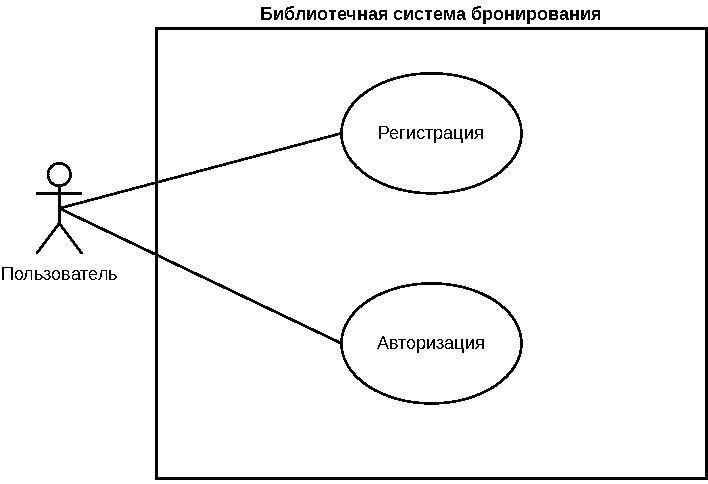
\includegraphics[scale = 1.1]{UseCaseUser}}
		\caption{Диаграмма прецедентов с точки зрения пользователя}
		\label{fig:use-case-user}
	\end{center}
\end{figure}

\newpage
\begin{landscape}
	\begin{figure}[h!]
		\center{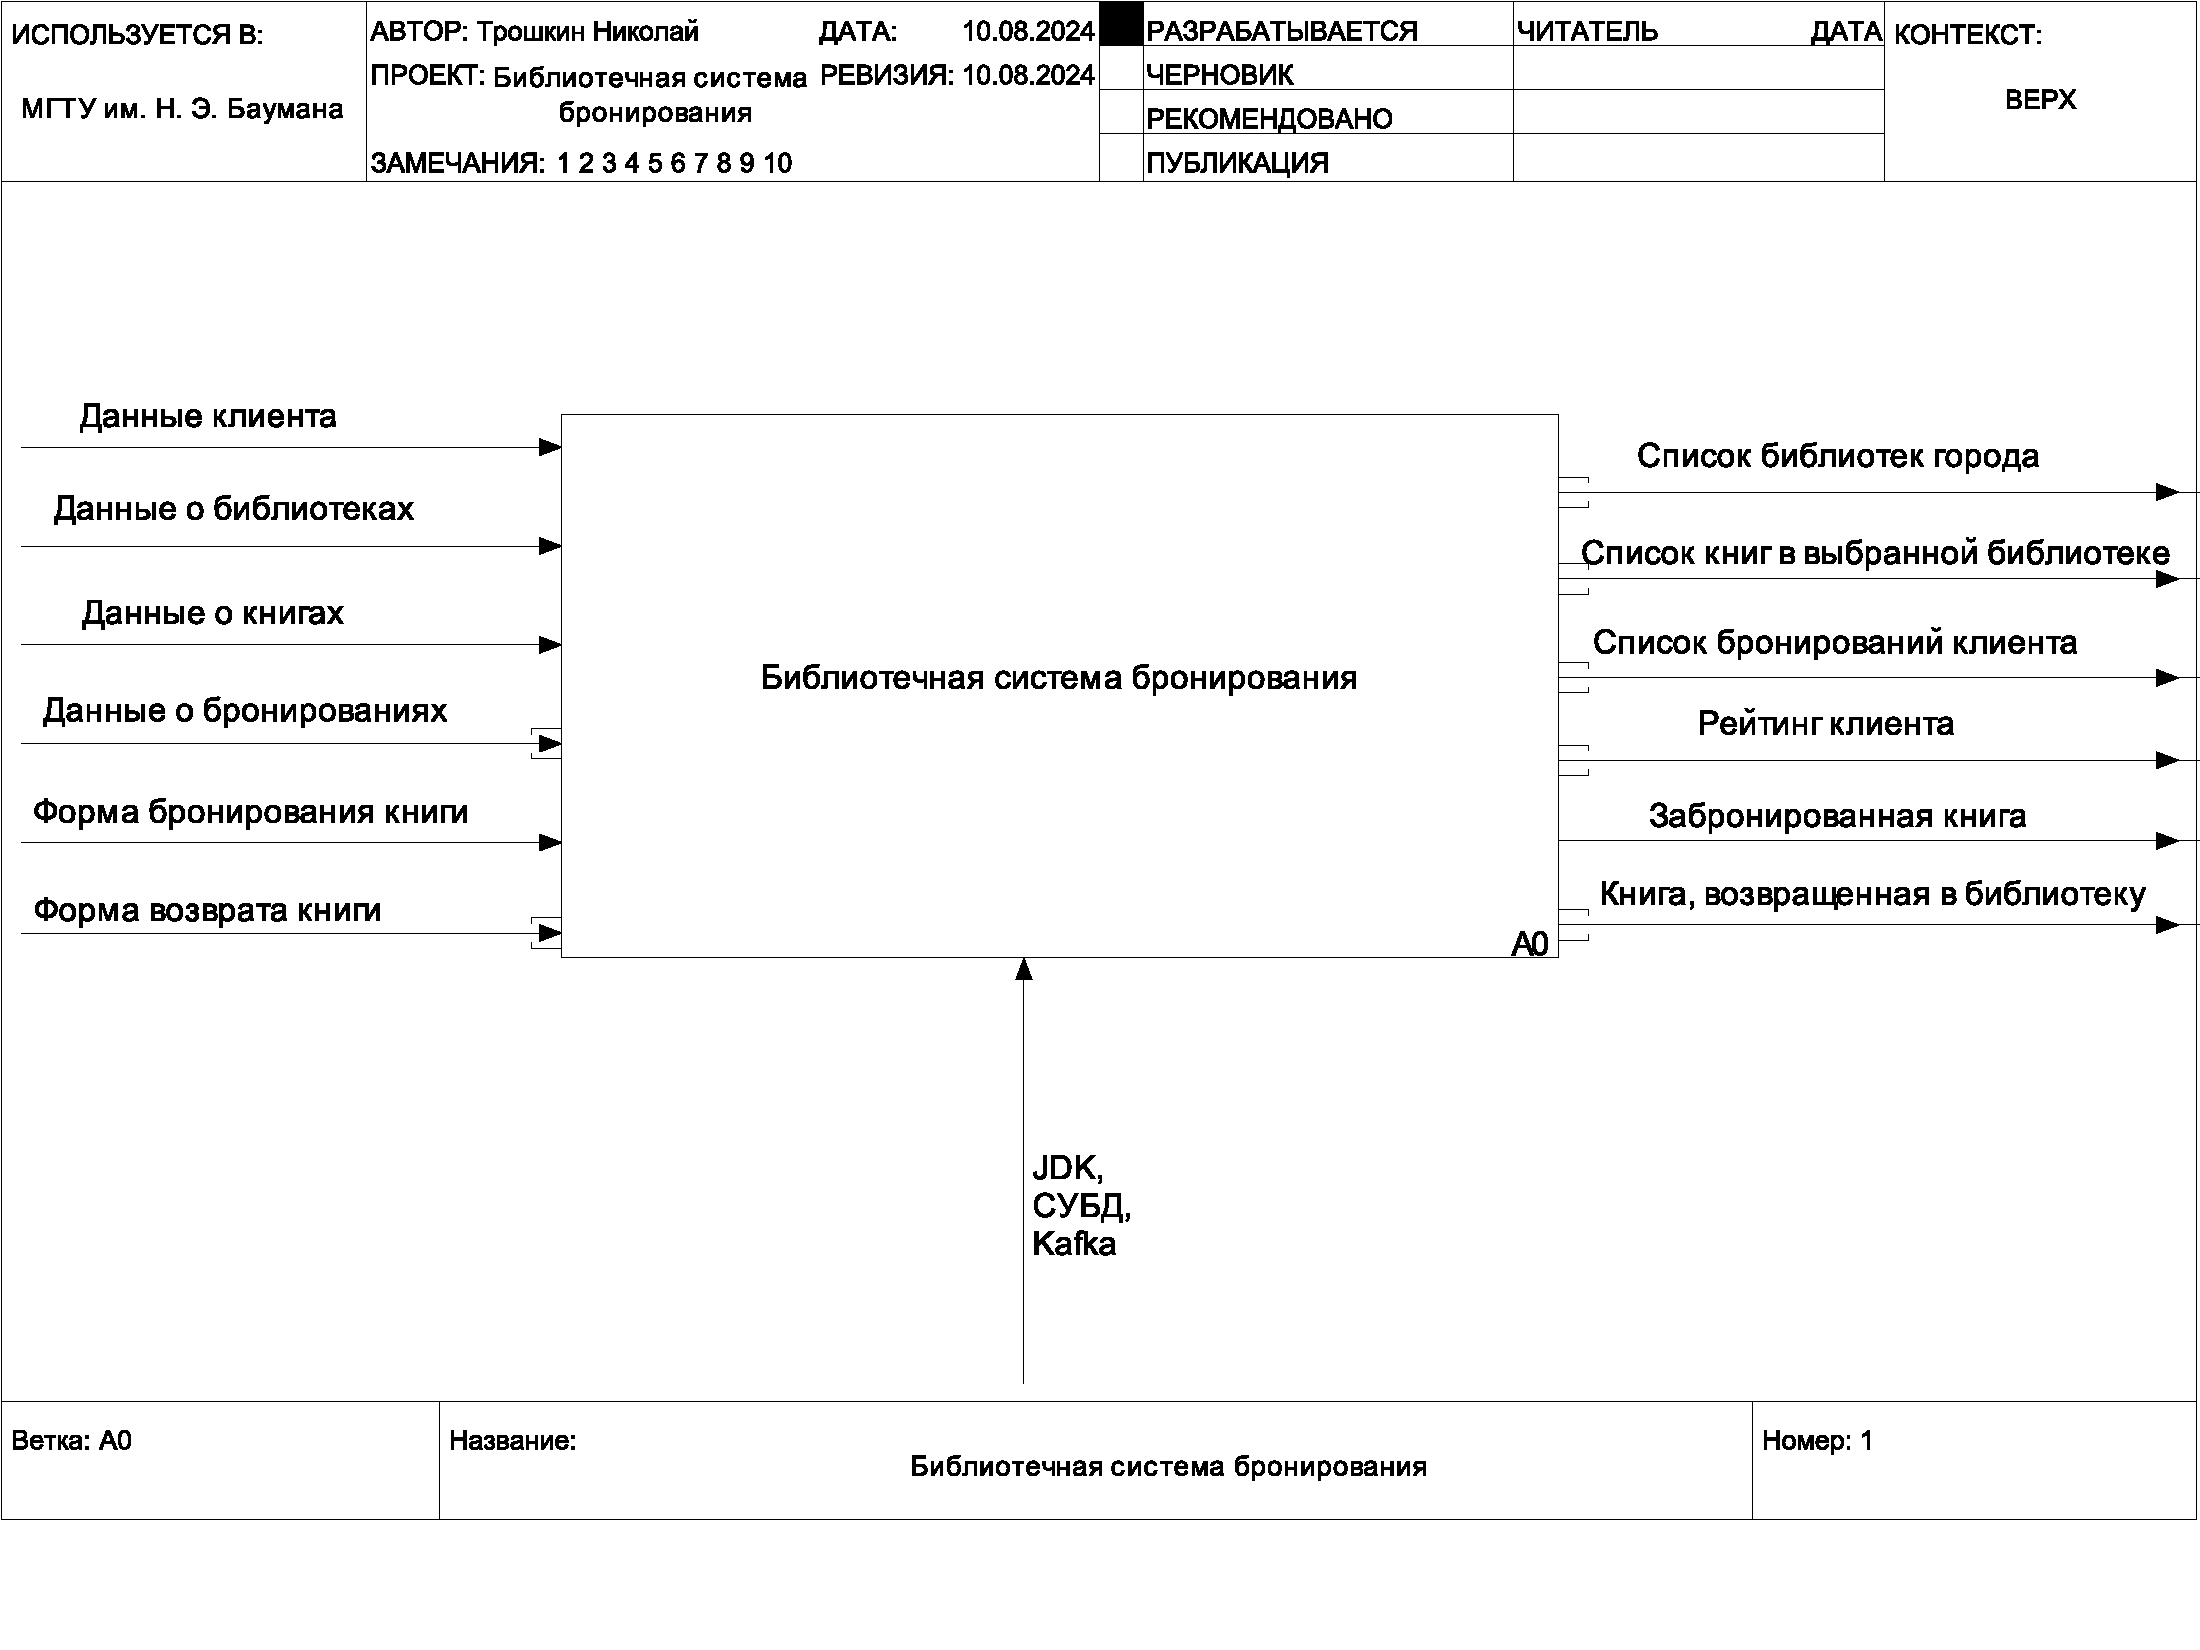
\includegraphics[scale = 0.57]{01_A0}}
		\caption{Концептуальная модуль системы в нотации IDEF0.}
		\label{fig:idef0-1}
	\end{figure}

	\begin{figure}[h!]
		\center{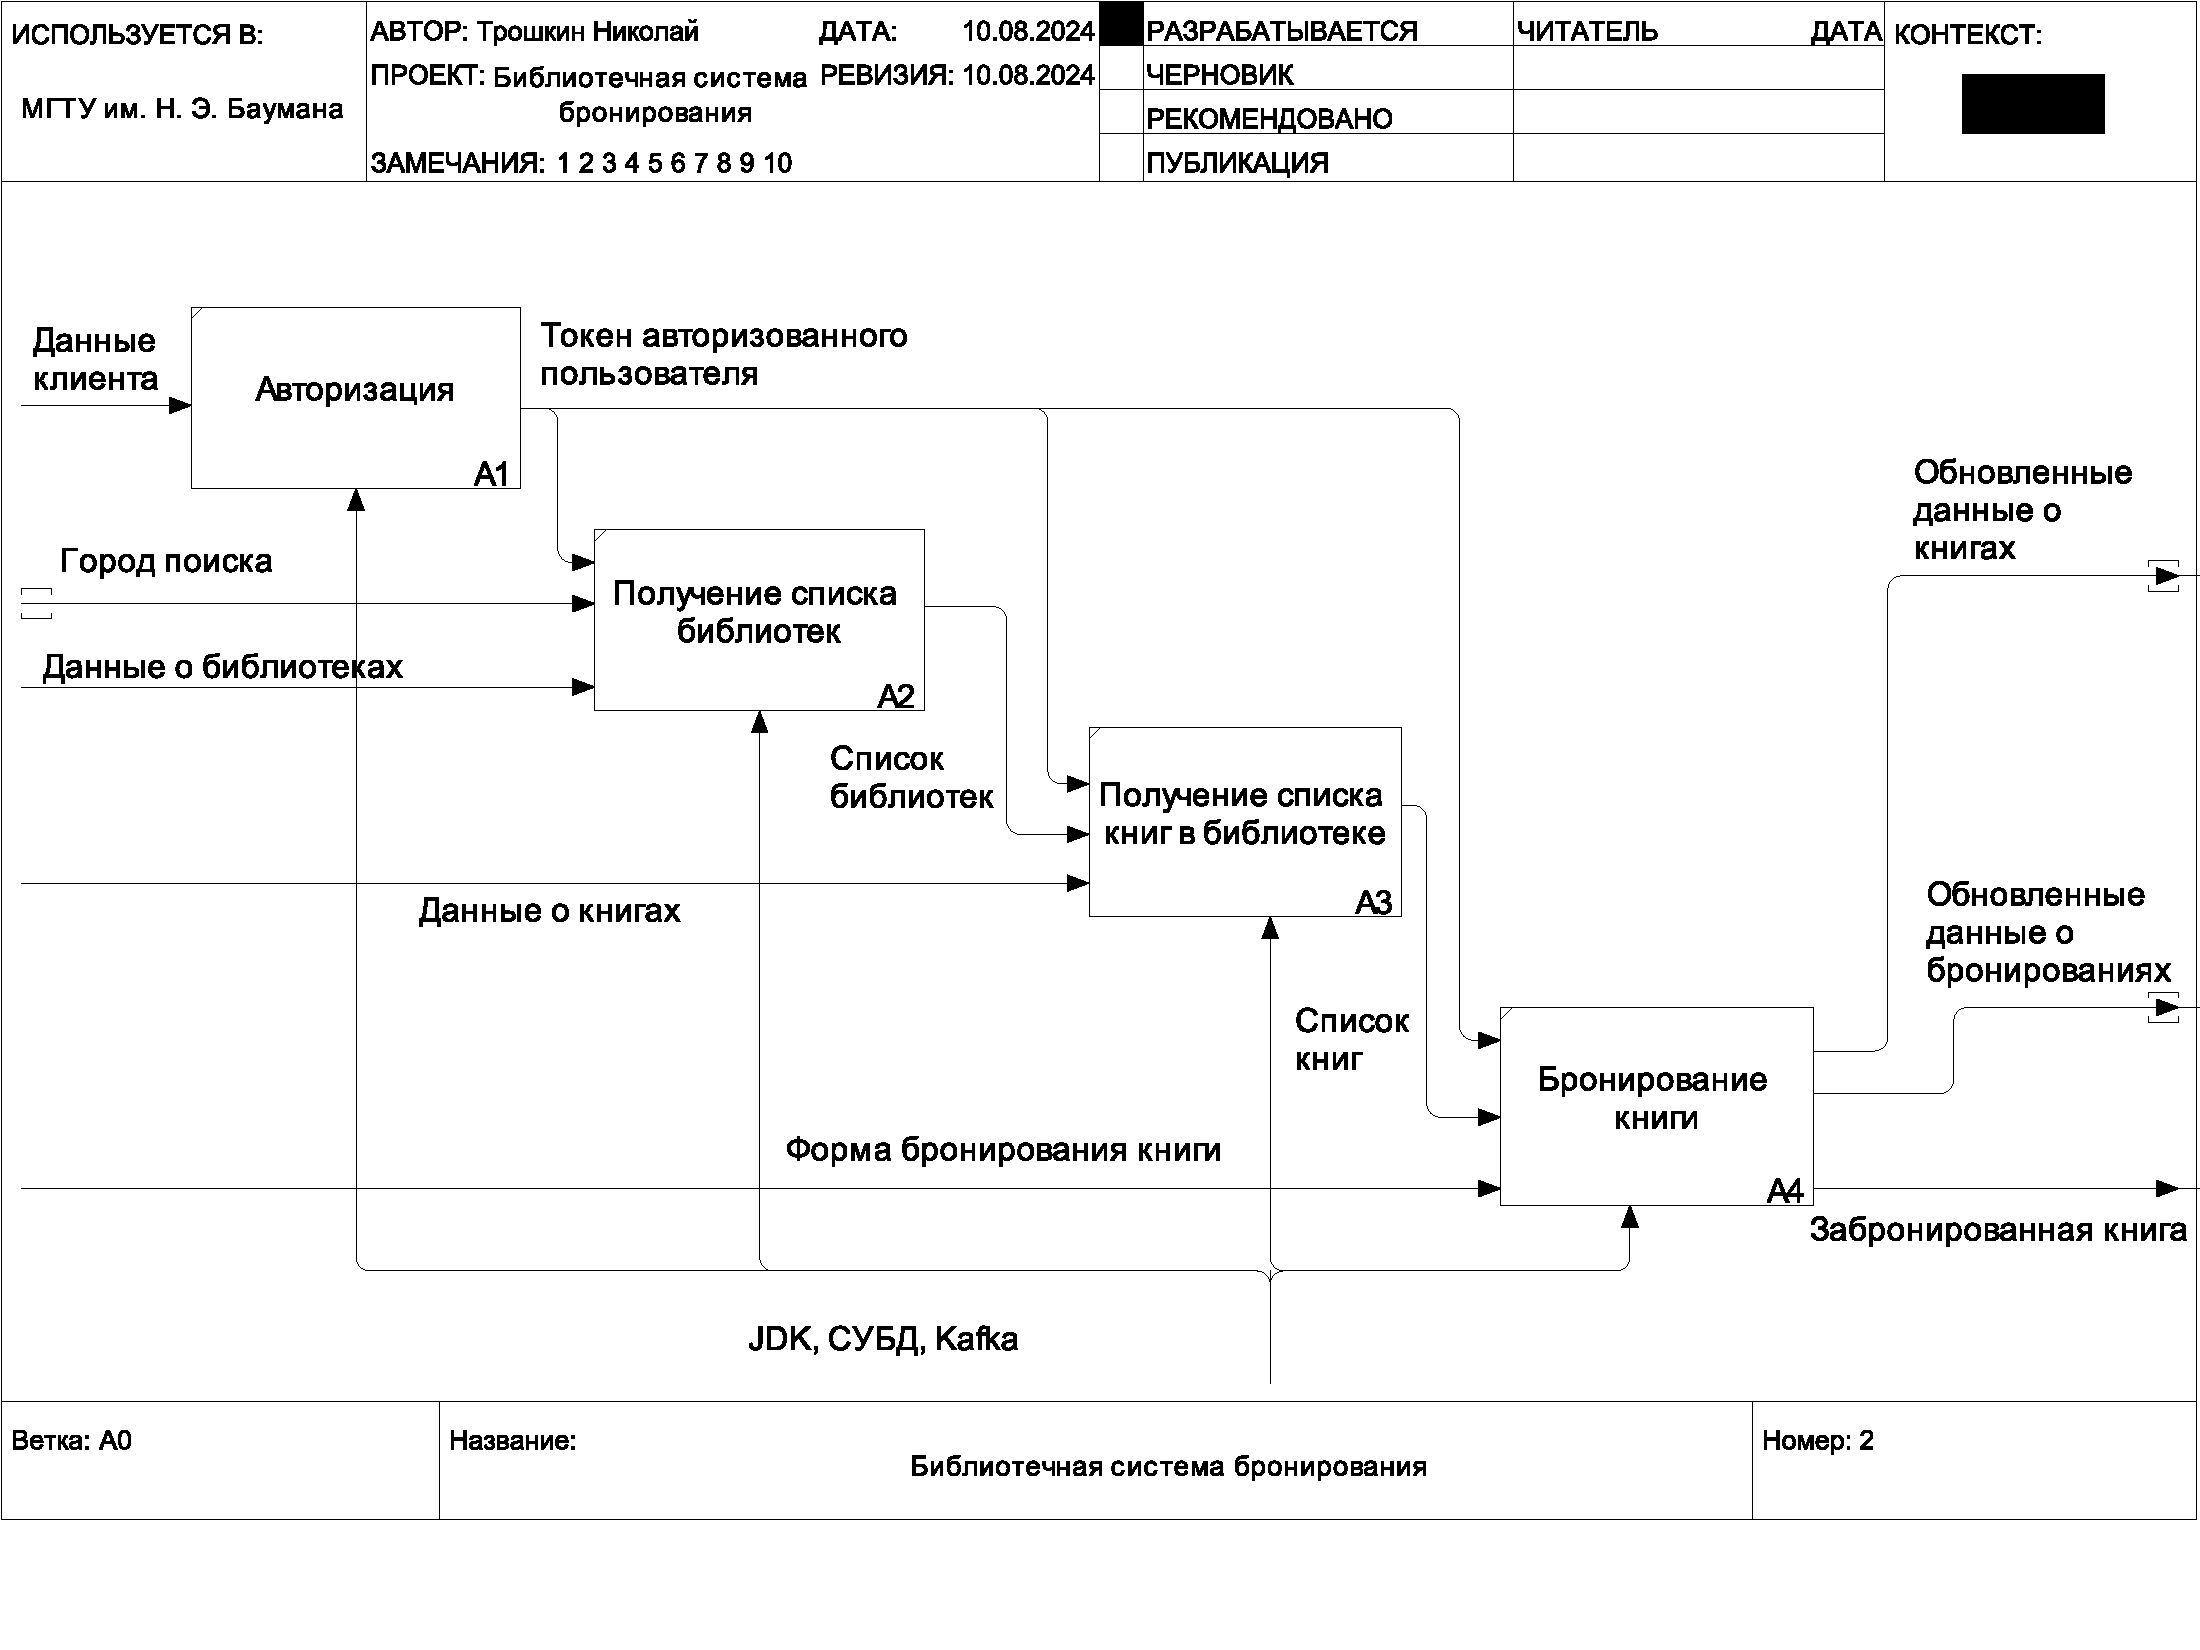
\includegraphics[scale = 0.57]{02_A0}}
		\caption{Детализированная концептуальная модель системы в нотации IDEF0.}
		\label{fig:idef0-2}
	\end{figure}
\end{landscape}


\begin{figure}[h]
	\begin{center}
		{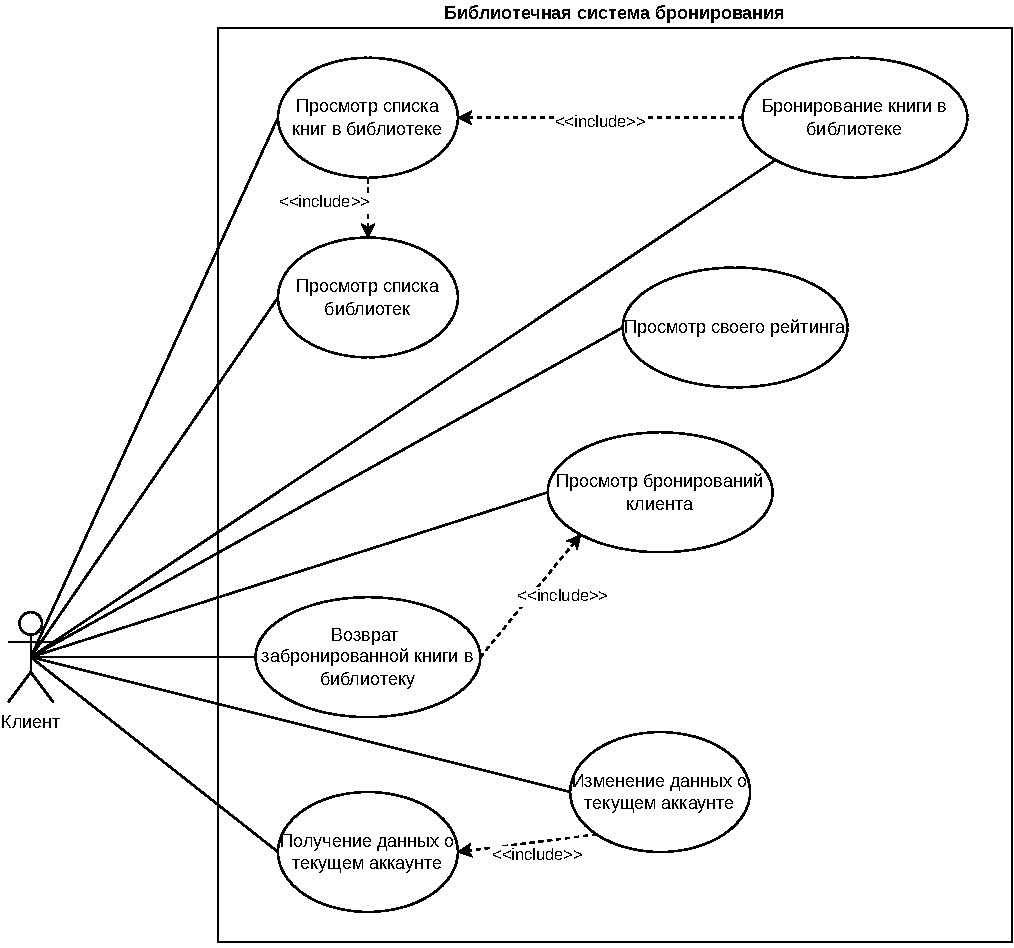
\includegraphics[scale = 0.6]{UseCaseClient}}
		\caption{Диаграмма прецедентов с точки зрения клиента.}
		\label{fig:use-case-client}
	\end{center}
\end{figure}

\begin{figure}[h!]
	\begin{center}
		{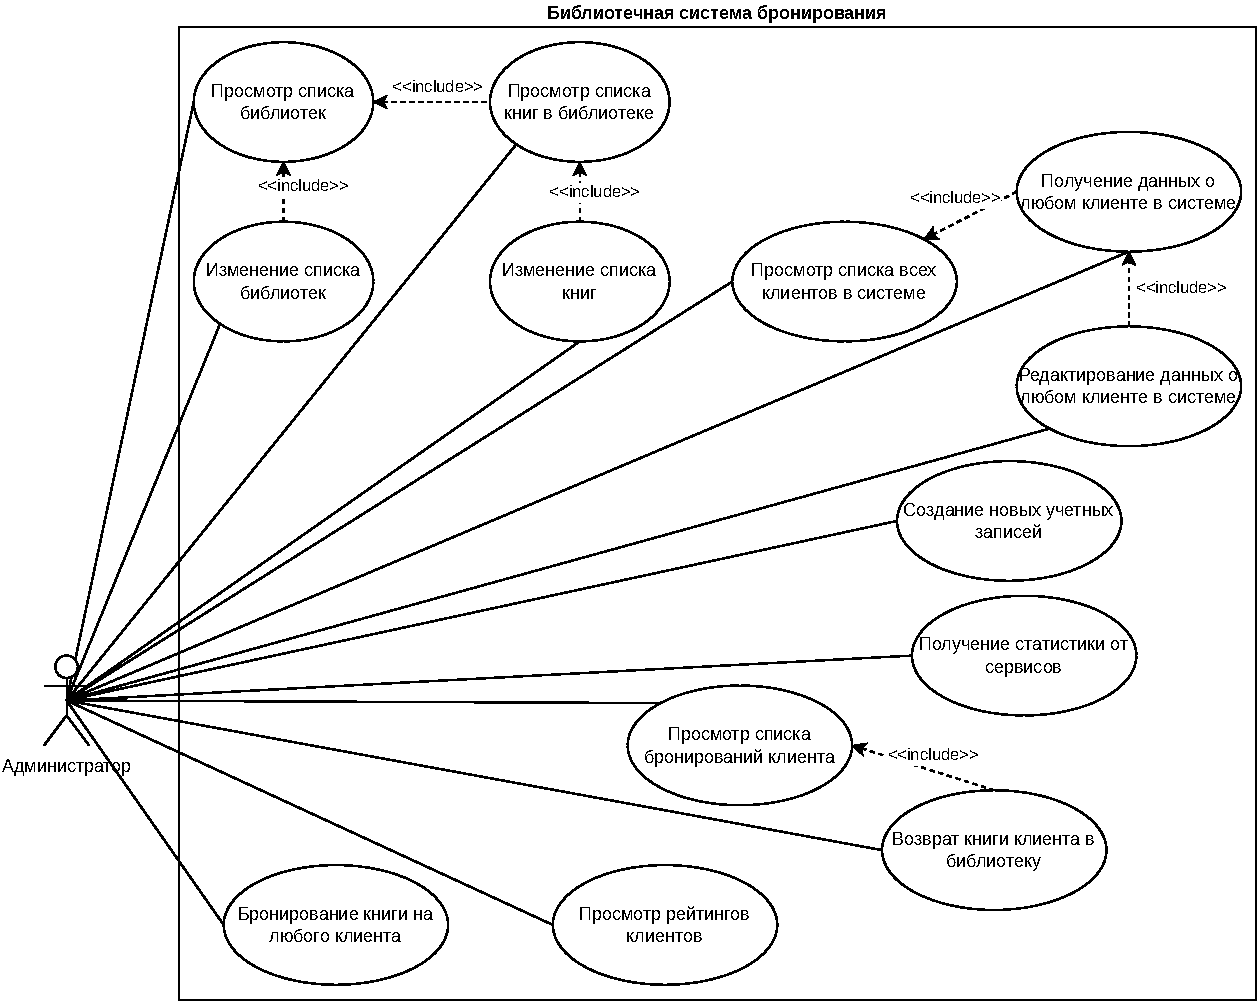
\includegraphics[scale = 0.6]{UseCaseAdmin}}
		\caption{Диаграмма прецедентов с точки зрения администратора.}
		\label{fig:use-case-admin}
	\end{center}
\end{figure}

\pagebreak

На рисунке \ref{fig:schema-reservation} представлена диаграмма деятельности в режиме <<Бронирование книги>> для клиента.

\begin{figure}[h!]
	\begin{center}
		{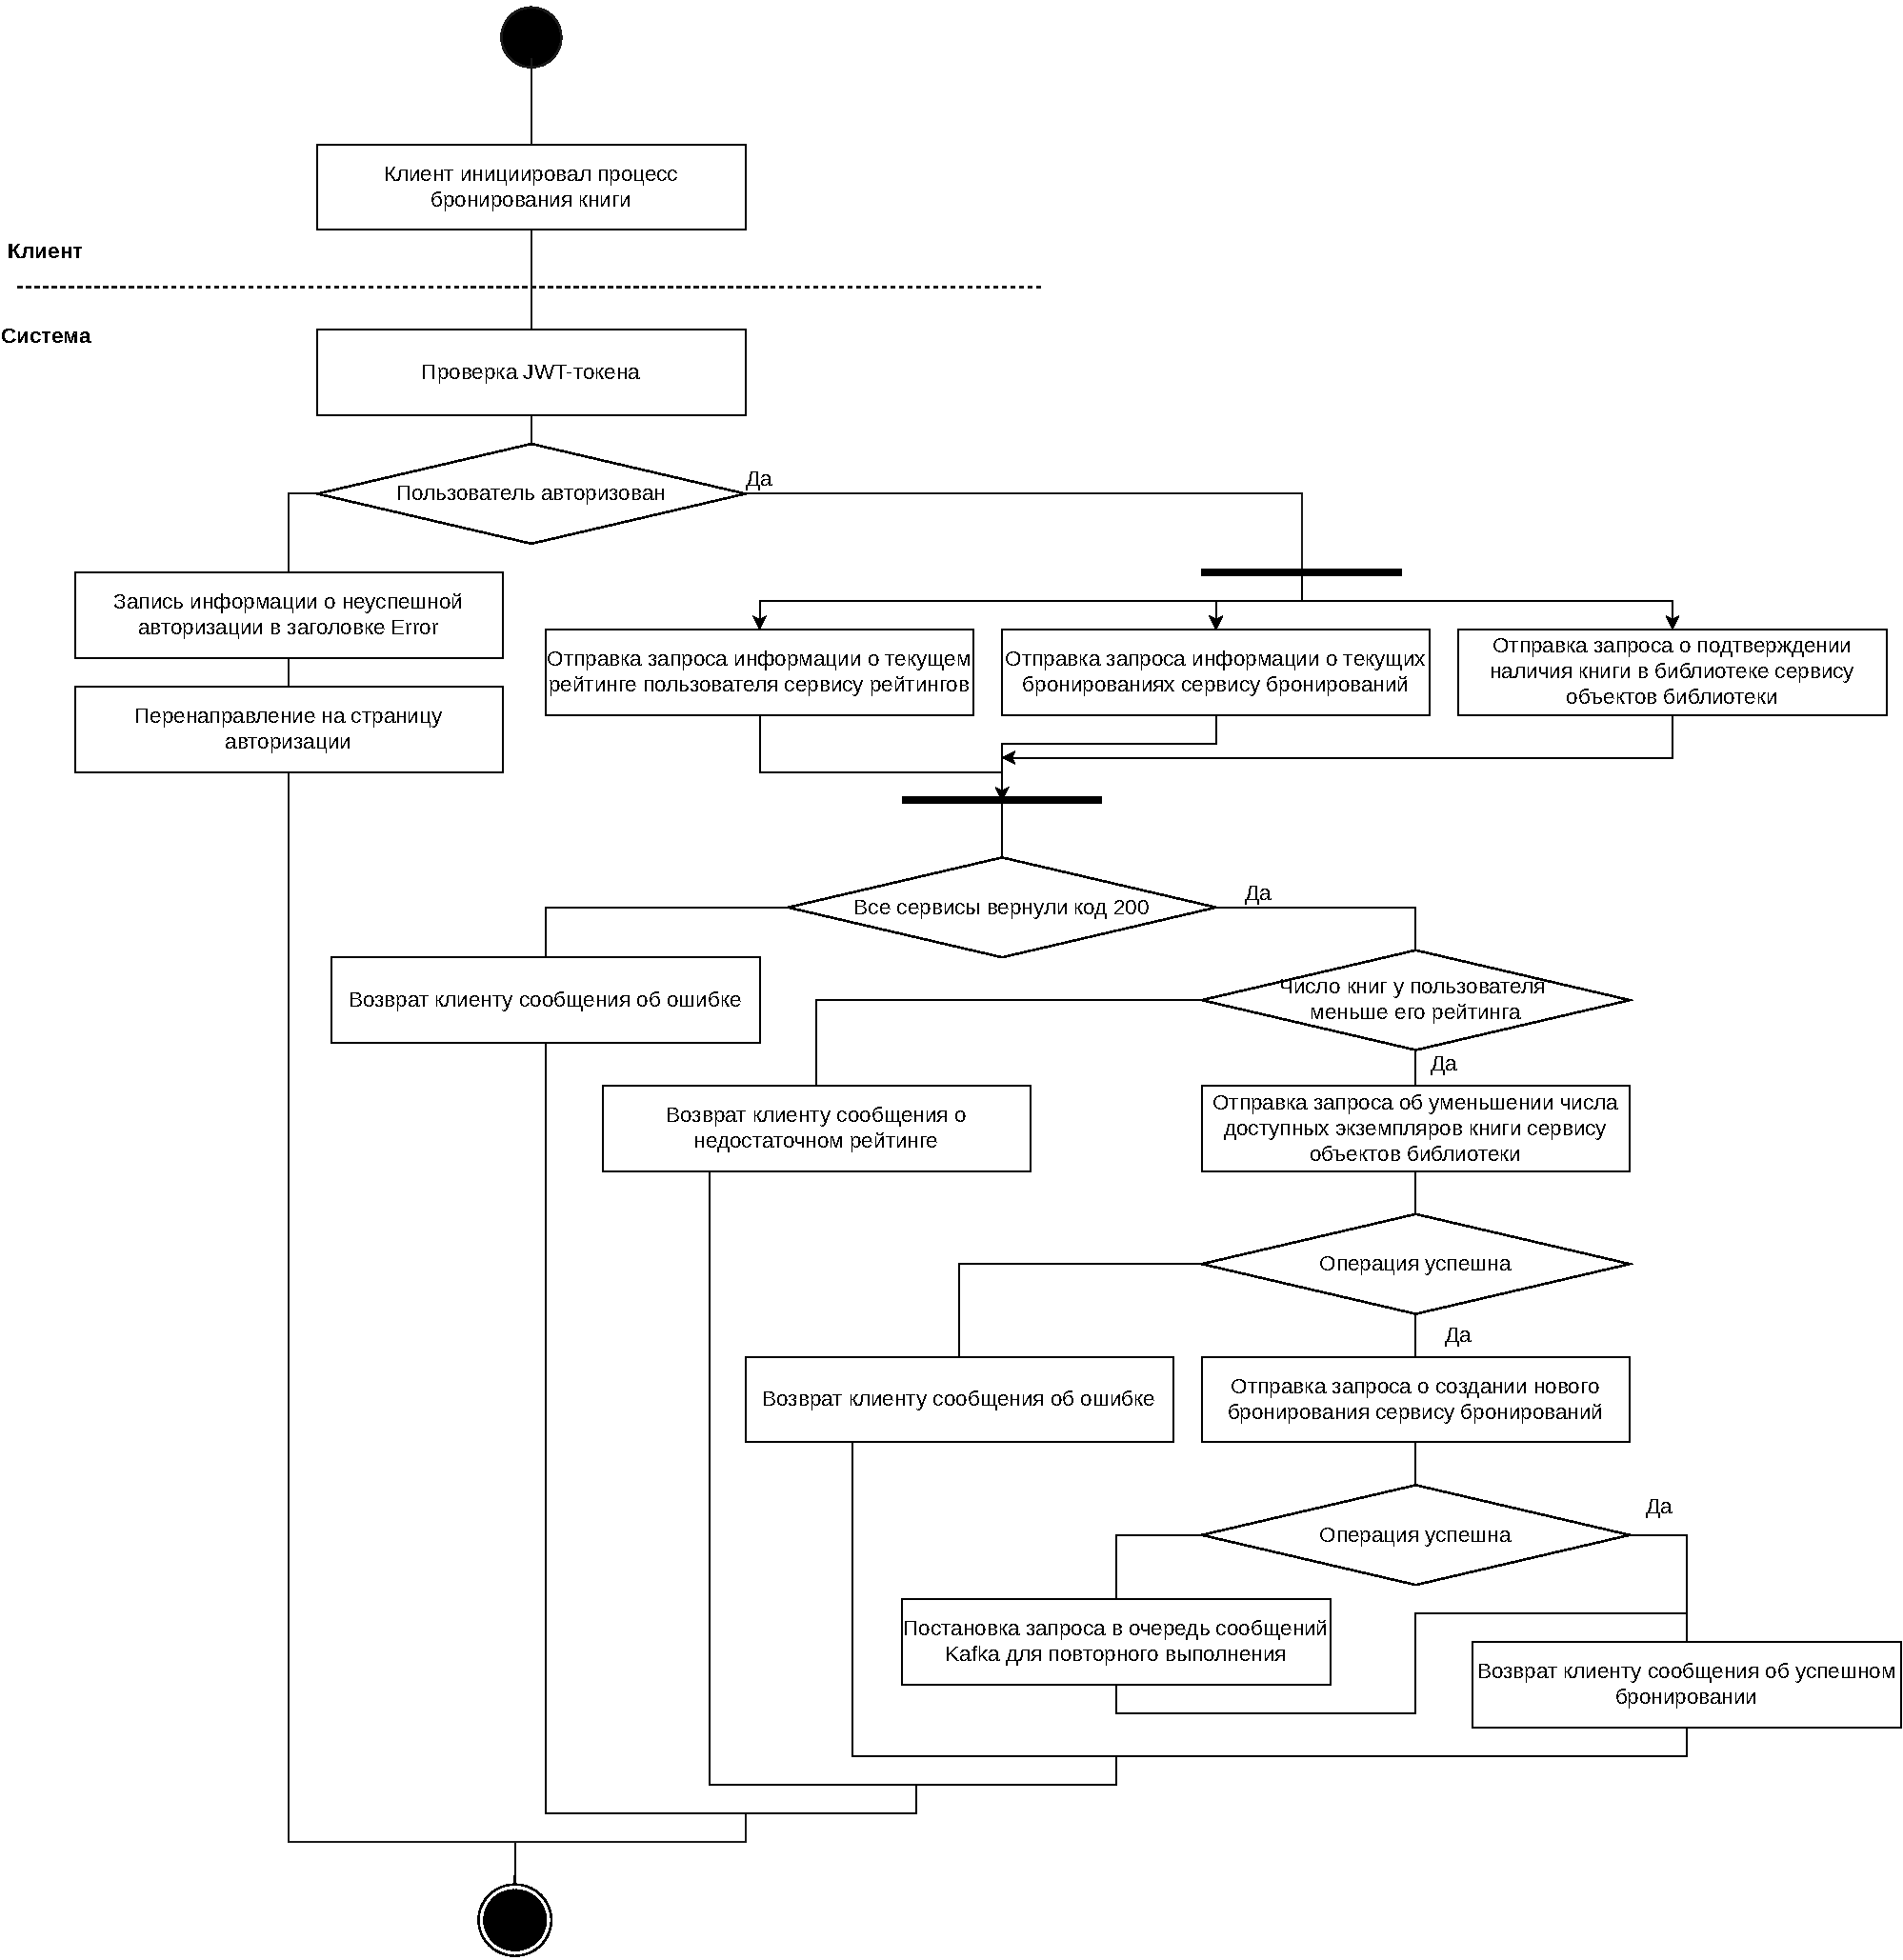
\includegraphics[scale = 0.5]{Activity}}
		\caption{Диаграмма деятельности в режиме <<Бронирование книги>> для клиента.}
		\label{fig:schema-reservation}
	\end{center}
\end{figure}

\pagebreak

\begin{landscape}

На рисунке \ref{fig:flow-level1} представлена наиболее важная для системы динамическая модель, представленная в виде диаграммы последовательности действий.

\begin{figure}[h!]
	\begin{center}
		{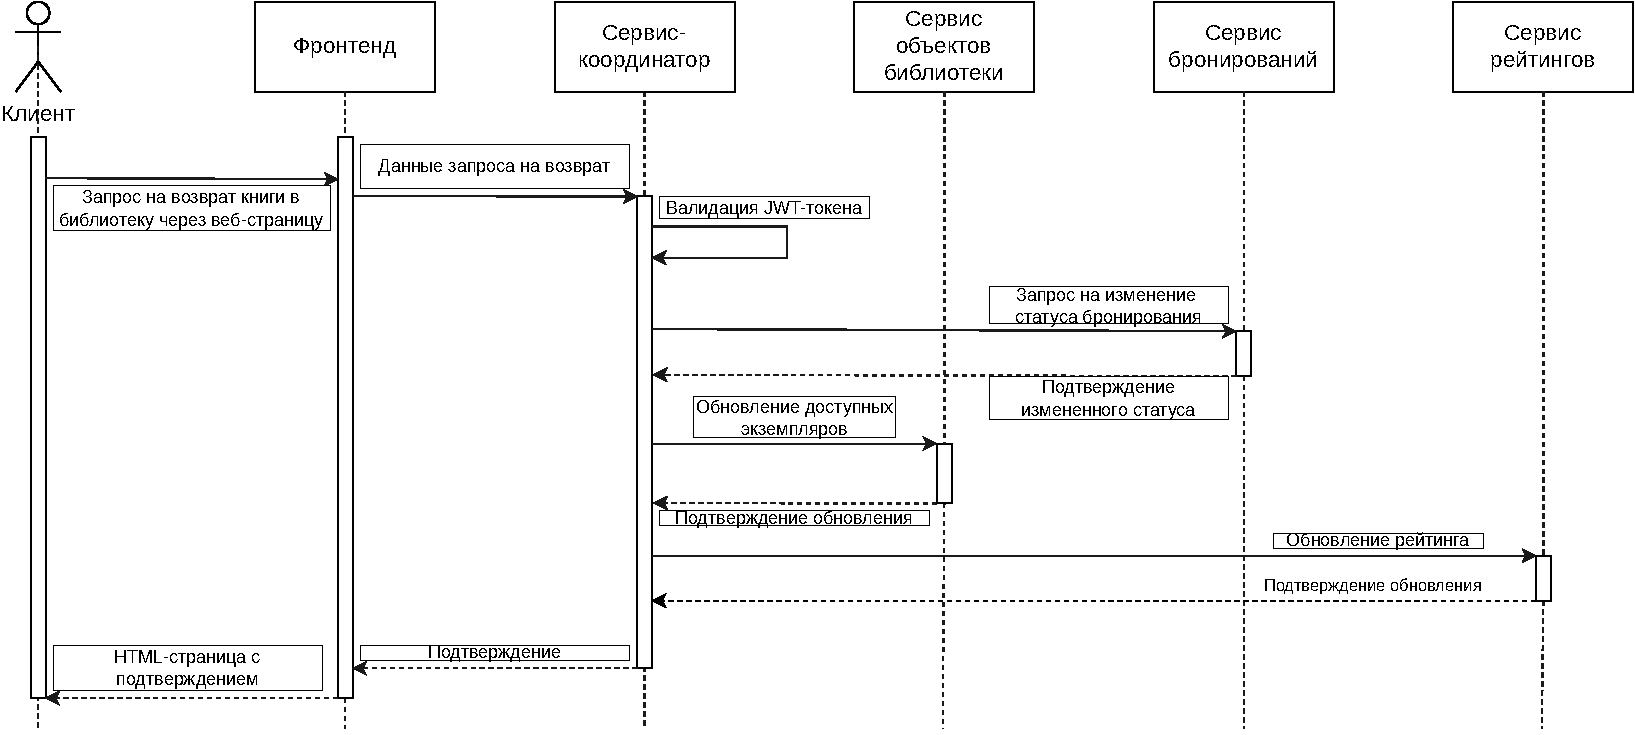
\includegraphics[scale = 0.9]{Sequence}}
		\caption{Диаграмма последовательности действий при возврате книги клиентом.}
		\label{fig:flow-level1}
	\end{center}
\end{figure}

\pagebreak
\end{landscape}

Диаграмма потоков данных, представленная на рисунке \ref{fig:data_flow}, позволяет описать распределение сохраняемой информации в хранилищах данных. Каждое хранилище данных будет реализовано в виде базы данных.

\begin{figure}[h!]
	\begin{center}
		{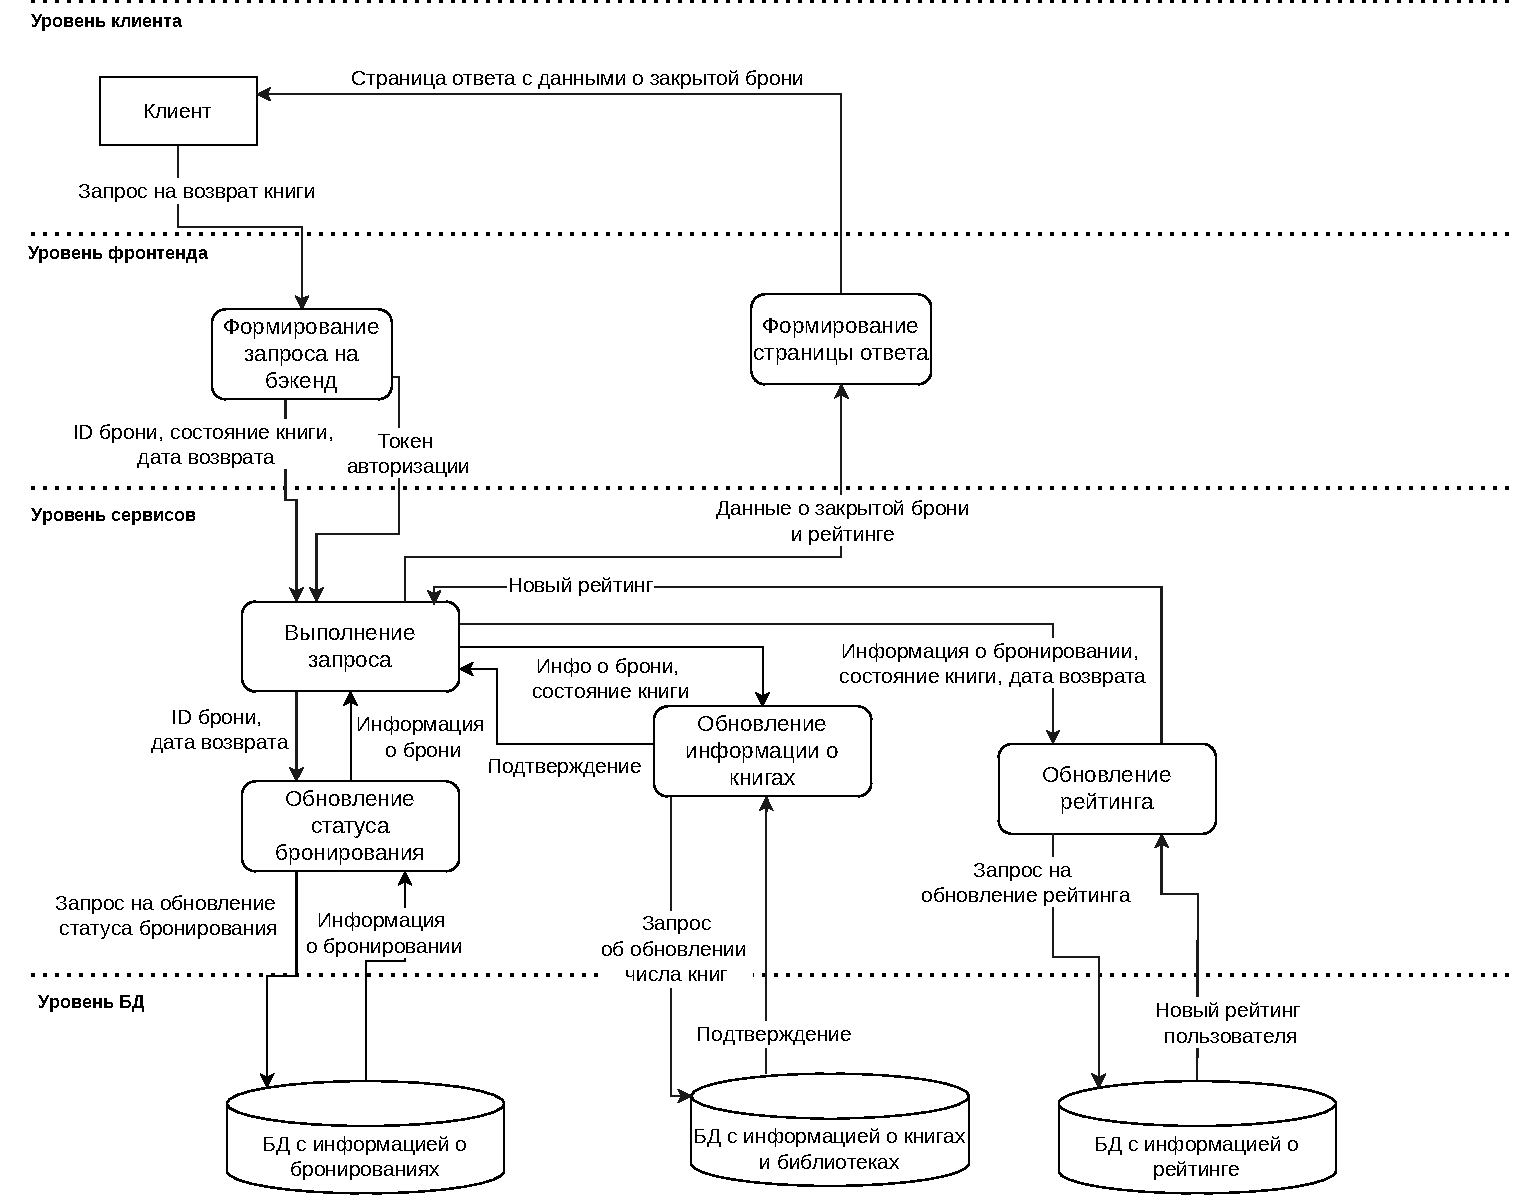
\includegraphics[scale = 0.75]{DataFlow}}
		\caption{Диаграмма потоков данных при возврате книги.}
		\label{fig:data_flow}
	\end{center}
\end{figure} 

\pagebreak

\subsection{Спецификация классов}
На рисунке \ref{fig:diag-classes} представлена диаграмма классов, принадлежащих основным компонентам микросервиса объектов библиотек.

\begin{figure}[h!]
	\begin{center}
		{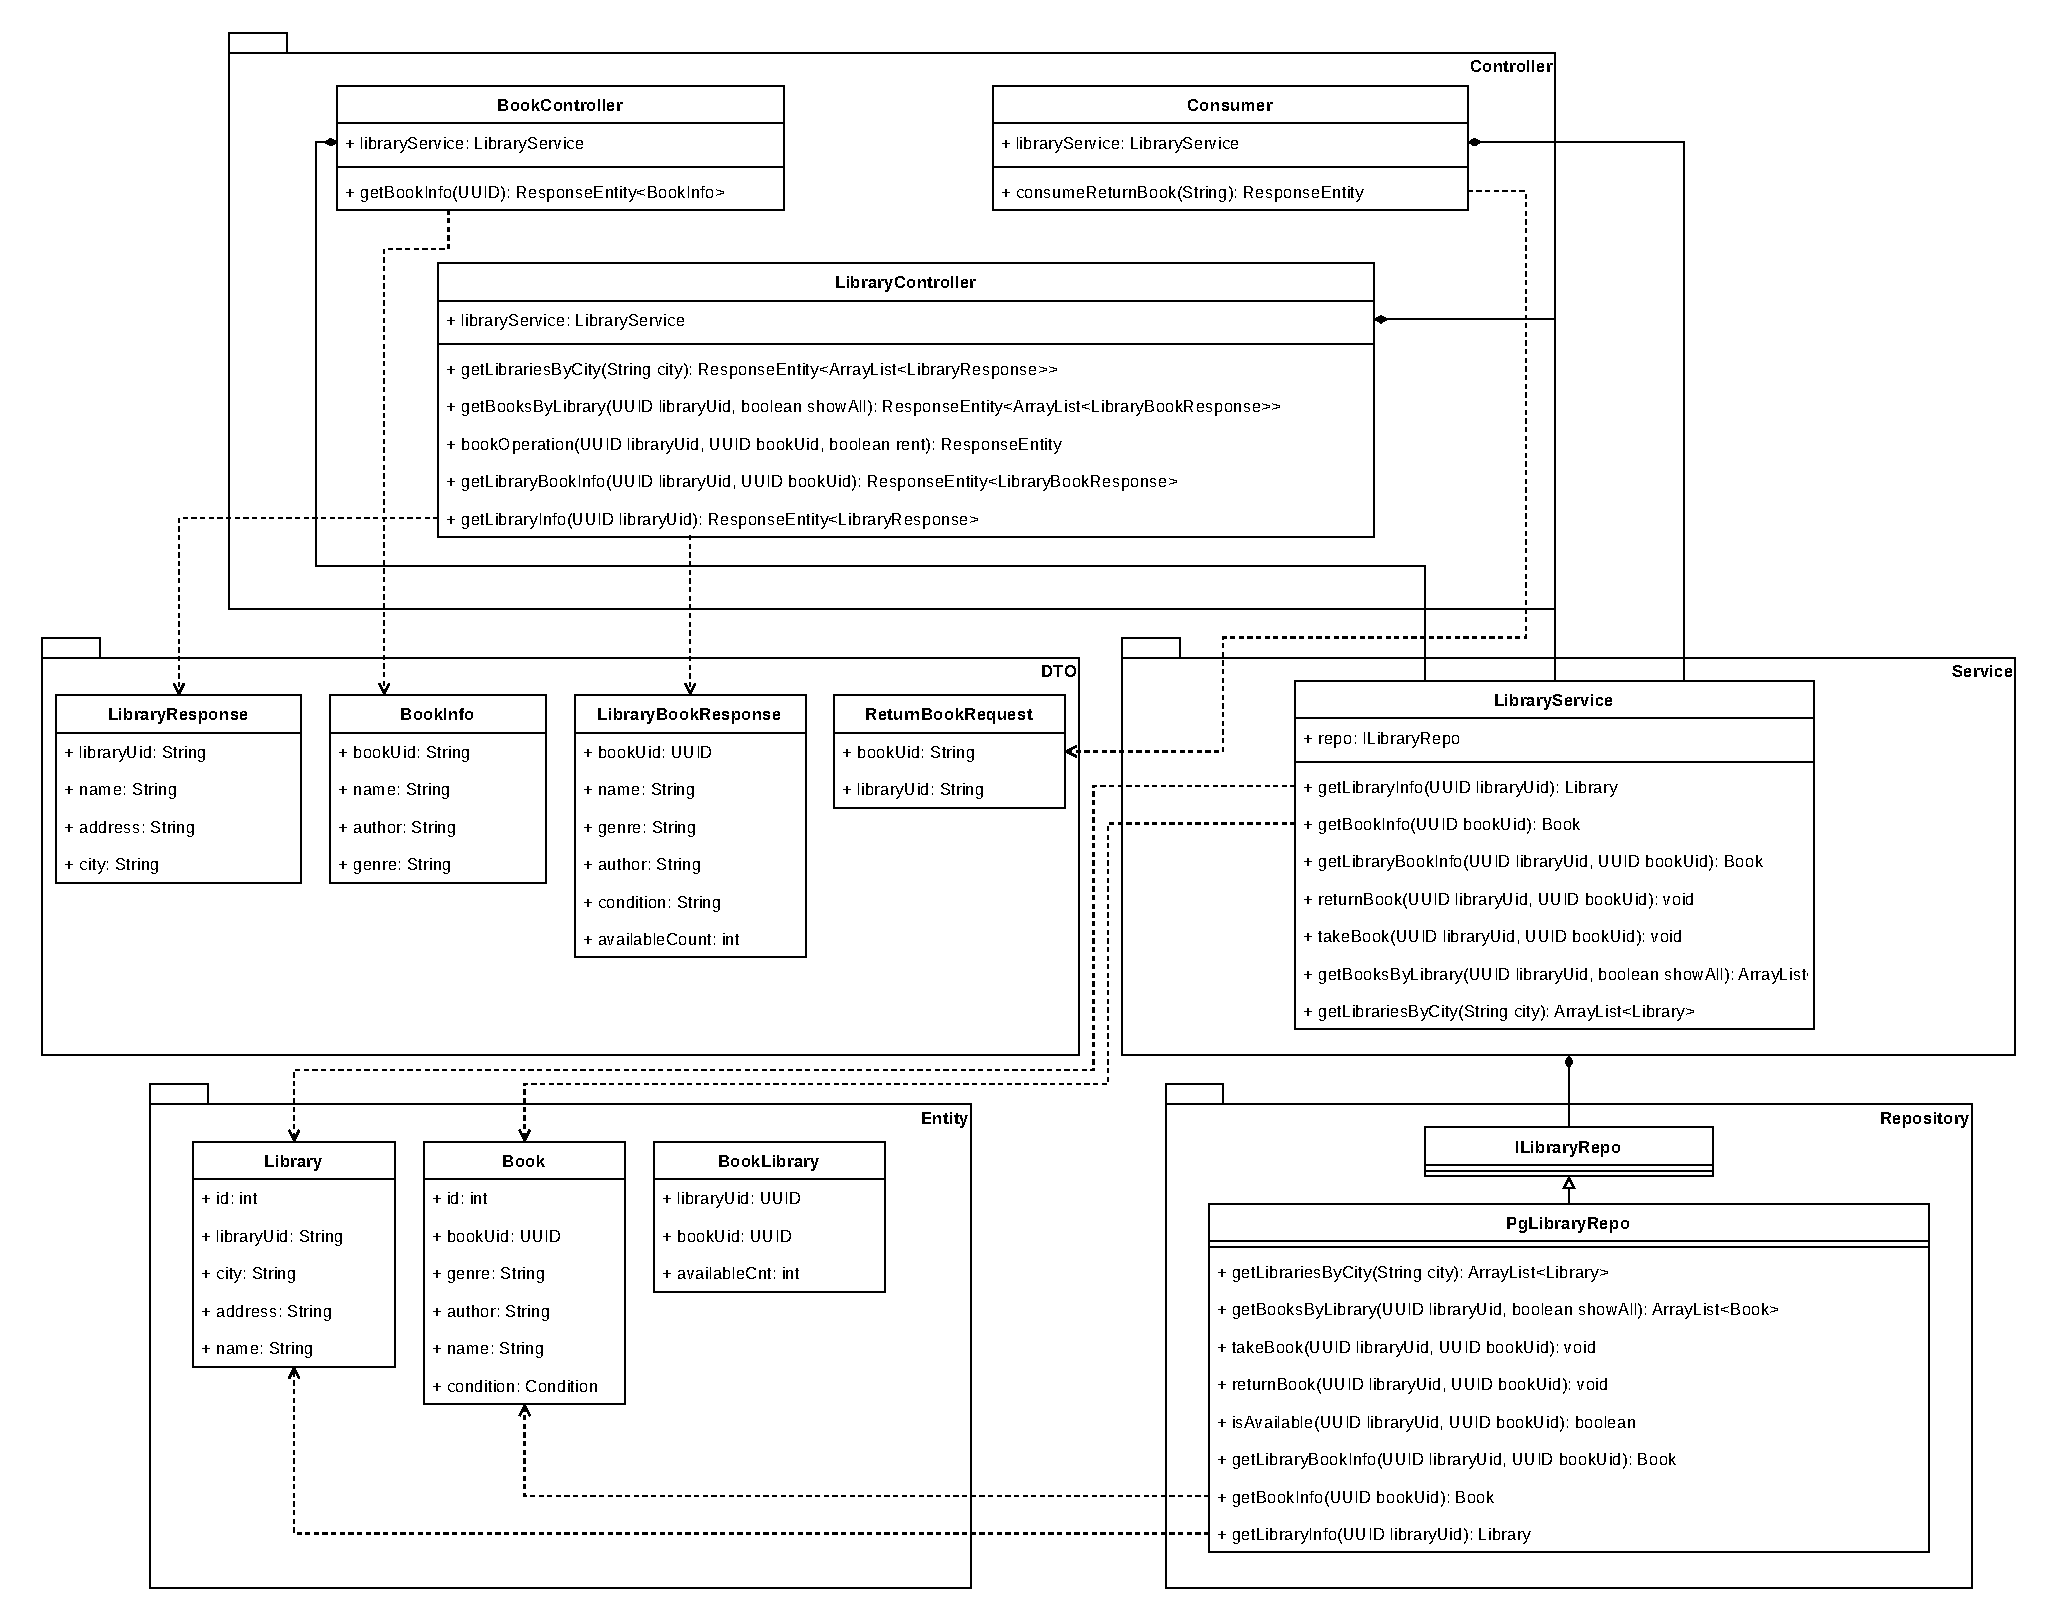
\includegraphics[scale = 0.5]{UML_Class}}
		\caption{Диаграмма классов}
		\label{fig:diag-classes}
	\end{center}
\end{figure}


Классы Library, Book, BookLibrary представляют легковесные объекты бизнес-логики, ассоциированные с соответствующими сущностями базы данных. 
Атрибуты указанных классов представлены в таблицах \ref{tbl:club}-\ref{tbl:registered}.

\begin{longtable}{| p{3cm} | p{5cm} | p{8cm} |}
	\caption{Атрибуты класса Library}
	\label{tbl:club} \\
	\hline
	
	\multicolumn{3}{|c|}{\textbf{Атрибуты}} \\
	\hline
	
	\textbf{Имя} & \textbf{Тип} & \textbf{Описание} \\
	\hline
	\endfirsthead
	
	\hline
	\textbf{Имя} & \textbf{Тип} & \textbf{Описание} \\
	\hline
	\endhead
	
	\hline
	\multicolumn{3}{c}{\textit{Продолжение на следующей странице}}
	\endfoot
	\hline
	\endlastfoot
	
	id
	&
	private: int
	&
	идентификатор библиотеки в БД\\
	\hline
	
	libraryUid
	&
	private: String
	&
	UUID библиотеки \\
	\hline
	
	address
	&
	private: String
	&
	адрес \\
	\hline

	city
	&
	private: String
	&
	город \\
	\hline
	
	name
	&
	private: String
	&
	название библиотеки \\
\end{longtable}

\begin{longtable}{| p{3cm} | p{5cm} | p{8cm} |}
	\caption{Атрибуты класса Book}
	\label{tbl:abonement} \\
	\hline
	
	\multicolumn{3}{|c|}{\textbf{Атрибуты}} \\
	\hline
	
	\textbf{Имя} & \textbf{Тип} & \textbf{Описание} \\
	\hline
	\endfirsthead
	
	\hline
	\textbf{Имя} & \textbf{Тип} & \textbf{Описание} \\
	\hline
	\endhead
	
	\hline
	\multicolumn{3}{c}{\textit{Продолжение на следующей странице}}
	\endfoot
	\hline
	\endlastfoot
	
	id
	&
	private: int
	&
	идентификатор книги в БД \\
	\hline
	
	bookUid
	&
	private: UUID
	&
	UUID книги \\
	\hline
	
	name
	&
	private: String
	&
	название книги \\
	\hline
	
	author
	&
	private: String
	&
	автор \\
	\hline
	
	genre
	&
	private: String
	&
	жанр книги \\
	\hline
	
	condition
	&
	private: Condition
	&
	состояние книги (enum: плохое, хорошее, отличное) \\
\end{longtable}

\begin{longtable}{| p{3cm} | p{5cm} | p{8cm} |}
	\caption{Атрибуты класса BookLibrary}
	\label{tbl:registered} \\
	\hline
	
	\multicolumn{3}{|c|}{\textbf{Атрибуты}} \\
	\hline
	
	\textbf{Имя} & \textbf{Тип} & \textbf{Описание} \\
	\hline
	\endfirsthead
	
	\hline
	\textbf{Имя} & \textbf{Тип} & \textbf{Описание} \\
	\hline
	\endhead
	
	\hline
	\multicolumn{3}{c}{\textit{Продолжение на следующей странице}}
	\endfoot
	\hline
	\endlastfoot
	
	libraryUid
	&
	private: UUID
	&
	UUID библиотеки \\
	\hline
	
	bookUid
	&
	private: UUID
	&
	UUID книги \\
	\hline
	
	availableCnt
	&
	private: int
	&
	количество доступных экземпляров данной книги в данной библиотеке \\
\end{longtable}

Классы LibraryResponse, BookInfo, LibraryBookResponse, ReturnBookRequest представляют объекты для передачи данных между сервисами. 
Атрибутивный состав LibraryResponse, BookInfo, LibraryBookResponse аналогичен составу ассоциированных с ними сущностей базы данных. 

Класс PgLibraryRepo отвечает за взаимодействие микросервиса с базой данных. 
Его методы приведены в таблице \ref{tbl:clubrepository}.

\begin{longtable}{| p{8cm} | p{8cm} |}
	\caption{Атрибуты класса PgLibraryRepo}
	\label{tbl:clubrepository} \\
	\hline
	
	\multicolumn{2}{|c|}{\textbf{Методы}} \\
	\hline
	
	\textbf{Название} & \textbf{Описание} \\
	\hline
	\endfirsthead
	
	\hline
	\textbf{Название} & \textbf{Описание} \\
	\hline
	\endhead
	
	\hline
	\multicolumn{2}{c}{\textit{Продолжение на следующей странице}}
	\endfoot
	\hline
	\endlastfoot
	
	getLibrariesByCity(String): Library[]
	&
	param: [String - in] - город \newline
	\textit{получение информации о библиотеках в городе}\\
	\hline
	
	getBooksByLibrary(UUID, boolean): Book[]
	&
	param: libraryUid [UUID - in] - идентификатор библиотеки  \newline
	param: showAll [boolean - in] - флаг, если установлен, получить даже книги, которых нет в наличии \newline
	\textit{получение информации о фитнес-клубе по его идентификатору}\\
	\hline
	
	takeBook(UUID, UUID): void
	&
	param: libraryUid [UUID - in] - идентификатор библиотеки  \newline
	param: bookUid [UUID - in] - идентификатор книги \newline
	\textit{уменьшение числа доступных экземпляров взятой книги в выбранной библиотеке}\\
	\hline
	
	returnBook(UUID, UUID): void
	&
	param: libraryUid [UUID - in] - идентификатор библиотеки  \newline
	param: bookUid [UUID - in] - идентификатор книги \newline
	\textit{увеличение числа доступных экземпляров возвращенной книги в библиотеке}\\
	\hline
	
	isAvailable(UUID, UUID): boolean
	&
	param: libraryUid [UUID - in] - идентификатор библиотеки  \newline
	param: bookUid [UUID - in] - идентификатор книги \newline
	\textit{проверка наличия книги в библиотеке}\\
	\hline
	
	getLibraryBookInfo(UUID, UUID): Book
	&
	param: libraryUid [UUID - in] - идентификатор библиотеки  \newline
	param: bookUid [UUID - in] - идентификатор книги \newline
	\textit{получение полной информации о книге в библиотеке}\\
	\hline
	
	getBookInfo(UUID): Book
	&
	param: bookUid [UUID - in] - идентификатор книги \newline
	\textit{получение полной информации о книге}\\
	\hline
	
	getLibraryInfo(UUID): Library
	&
	param: libraryUid [UUID - in] - идентификатор библиотеки  \newline
	\textit{получение полной информации о библиотеке}\\
\end{longtable}

Класс LibraryService реализует бизнес-логику микросервиса, преобразование данных и передачу их на последующий слой, непосредственно связанный с базой данных, поэтому предоставляемые им методы схожи с методами класса PgLibraryRepo.

Классы LibraryController, BookController выполняют функцию преобразования транспортных сущностей в сущности базы данных и передачу запроса на уровень сервисов, а также формирование HTTP-ответа.
Класс Consumer отвечает за обработку очереди сообщений в Kafka, куда попадают не обработанные сразу запросы о возврате книги.

\newpage

\section{Технологический раздел}
\subsection{Средства разработки}
\subsubsection{Выбор СУБД}

В  соответствии  с  техническим  заданием  разработка  бекенда предусматривает следующие требования.
\begin{itemize}
	\item[---] \textbf{Безопасность  хранения  данных}.  Несанкционированный  доступ к данным клиентам должен быть невозможен.
	
	\item[---] \textbf{Транзакционность}.  Должен  соблюдаться  принцип  «ACID» (Atomicity  —  Атомарность,  Consistency  —  Согласованность, Isolation — Изолированность, Durability — Надежность). Атомарность гарантирует, что транзакция не может быть зафиксирована частично.  Согласованность  —  что  успешное  завершение  транзакции оставит  систему  в  согласованном состоянии. Изолированность  —  что  параллельно  выполняемые  транзакции  не  будут влиять друг на друга. Надежность — что успешно завершенная транзакция  будет  зафиксирована,  а  в случае  сбоя, после восстановления системы, результаты транзакции не будут утеряны.
	
	\item[---] \textbf{Масштабируемость}.  Выбранная  СУБД  должна  поддерживать репликацию, шардирование.
\end{itemize}

PostgreSQL [10] --- реляционная система управления базами данных. 
Она является некоммерческим ПО с открытым исходным кодом. 
Для работы с этой СУБД существуют библиотеки для таких распространенных языков программирования, как Python, Ruby, Perl, PHP, C, C++, Java, C\#, Go. 
Она работает под управлением многих операционных систем: Linux, MacOS, Windows, Solaris и др. 
По сравнению с MySQL система PostgreSQL лучше работает с репликацией, так как в ней существует журнал (средство восстановления системы в случае сбоя) физической модификации страниц. 
PostgreSQL осуществляет асинхронную репликацию типа «ведущий — ведомый».

Выбор СУБД PostgreSQL для хранения данных разрабатываемой системы обеспечит надежность, безопасность и масштабируемость. \\

\subsubsection{Средства разработки Identity Provider}
Для реализации функций Identity Provider используется Keycloak [11].
Это открытая платформа для управления идентификацией и доступом, которая позволяет разработчикам и администраторам легко управлять пользователями, ролями и доступом к различным приложениям.
На Keycloak переложены аутентификация, хранение данных о пользователях и управление сессиями.
Получение токенов, создание пользователей администратором и выход из учетной записи выполняются сервисом авторизации путем отправки соответствующих HTTP-запросов в Keycloak.

\subsubsection{Средства развертывания приложения}
Первоначально для развертывания приложения была выбрана платформа VK Cloud [12].
Это облачная платформа, предоставляемая компанией VK, которая предлагает различные облачные сервисы и решения для разработчиков. 
Платформа ориентирована на предоставление гибких и масштабируемых инфраструктурных ресурсов, таких как вычислительные мощности, хранилища данных, базы данных, сетевые решения и инструменты для развертывания приложений, в частности, управляемые кластеры Kubernetes.
Однако на каждого пользователя выделяется квота в 4 машины и 16 ГБ суммарной оперативной памяти.
На мастер-узел кластера требуется минимум 6 ГБ RAM.
На рабочих узлах требовалось развернуть 15 подов --- 6 сервисов, 4 базы данных, 3 пода для работы Kafka, клиентская часть приложения и Keycloak.
Были проверены следующие конфигурации:
\begin{enumerate}
	\item 2 рабочих узла с 4 ГБ оперативной памяти в каждом. Конфигурация не подошла, так как на ней можно было развернуть максимум 8 подов, этого не хватает даже, чтобы развернуть только бэкенд (все остальное можно было поднять на свободной машине в контейнере Docker).
	\item 3 рабочих узла с 2 ГБ оперативной памяти в каждом. Такая конфигурация также не подошла, так как узлы не выдерживали нагрузки и их требовалось постоянно перезагружать.
	\item Остальные возможные конфигурации выходили за рамки квот.
\end{enumerate}

Таким образом, пришлось отказаться от разворачивания приложения в облаке и для деплоя был выбран minikube [13], который позволяет развернуть кластер Kubernetes локально.

\subsection{Интерфейс программы}
На рисунке \ref{fig:interface} приведен пример web-страницы интерфейса разработанного приложения.
\begin{figure}[h!]
	\begin{center}
		{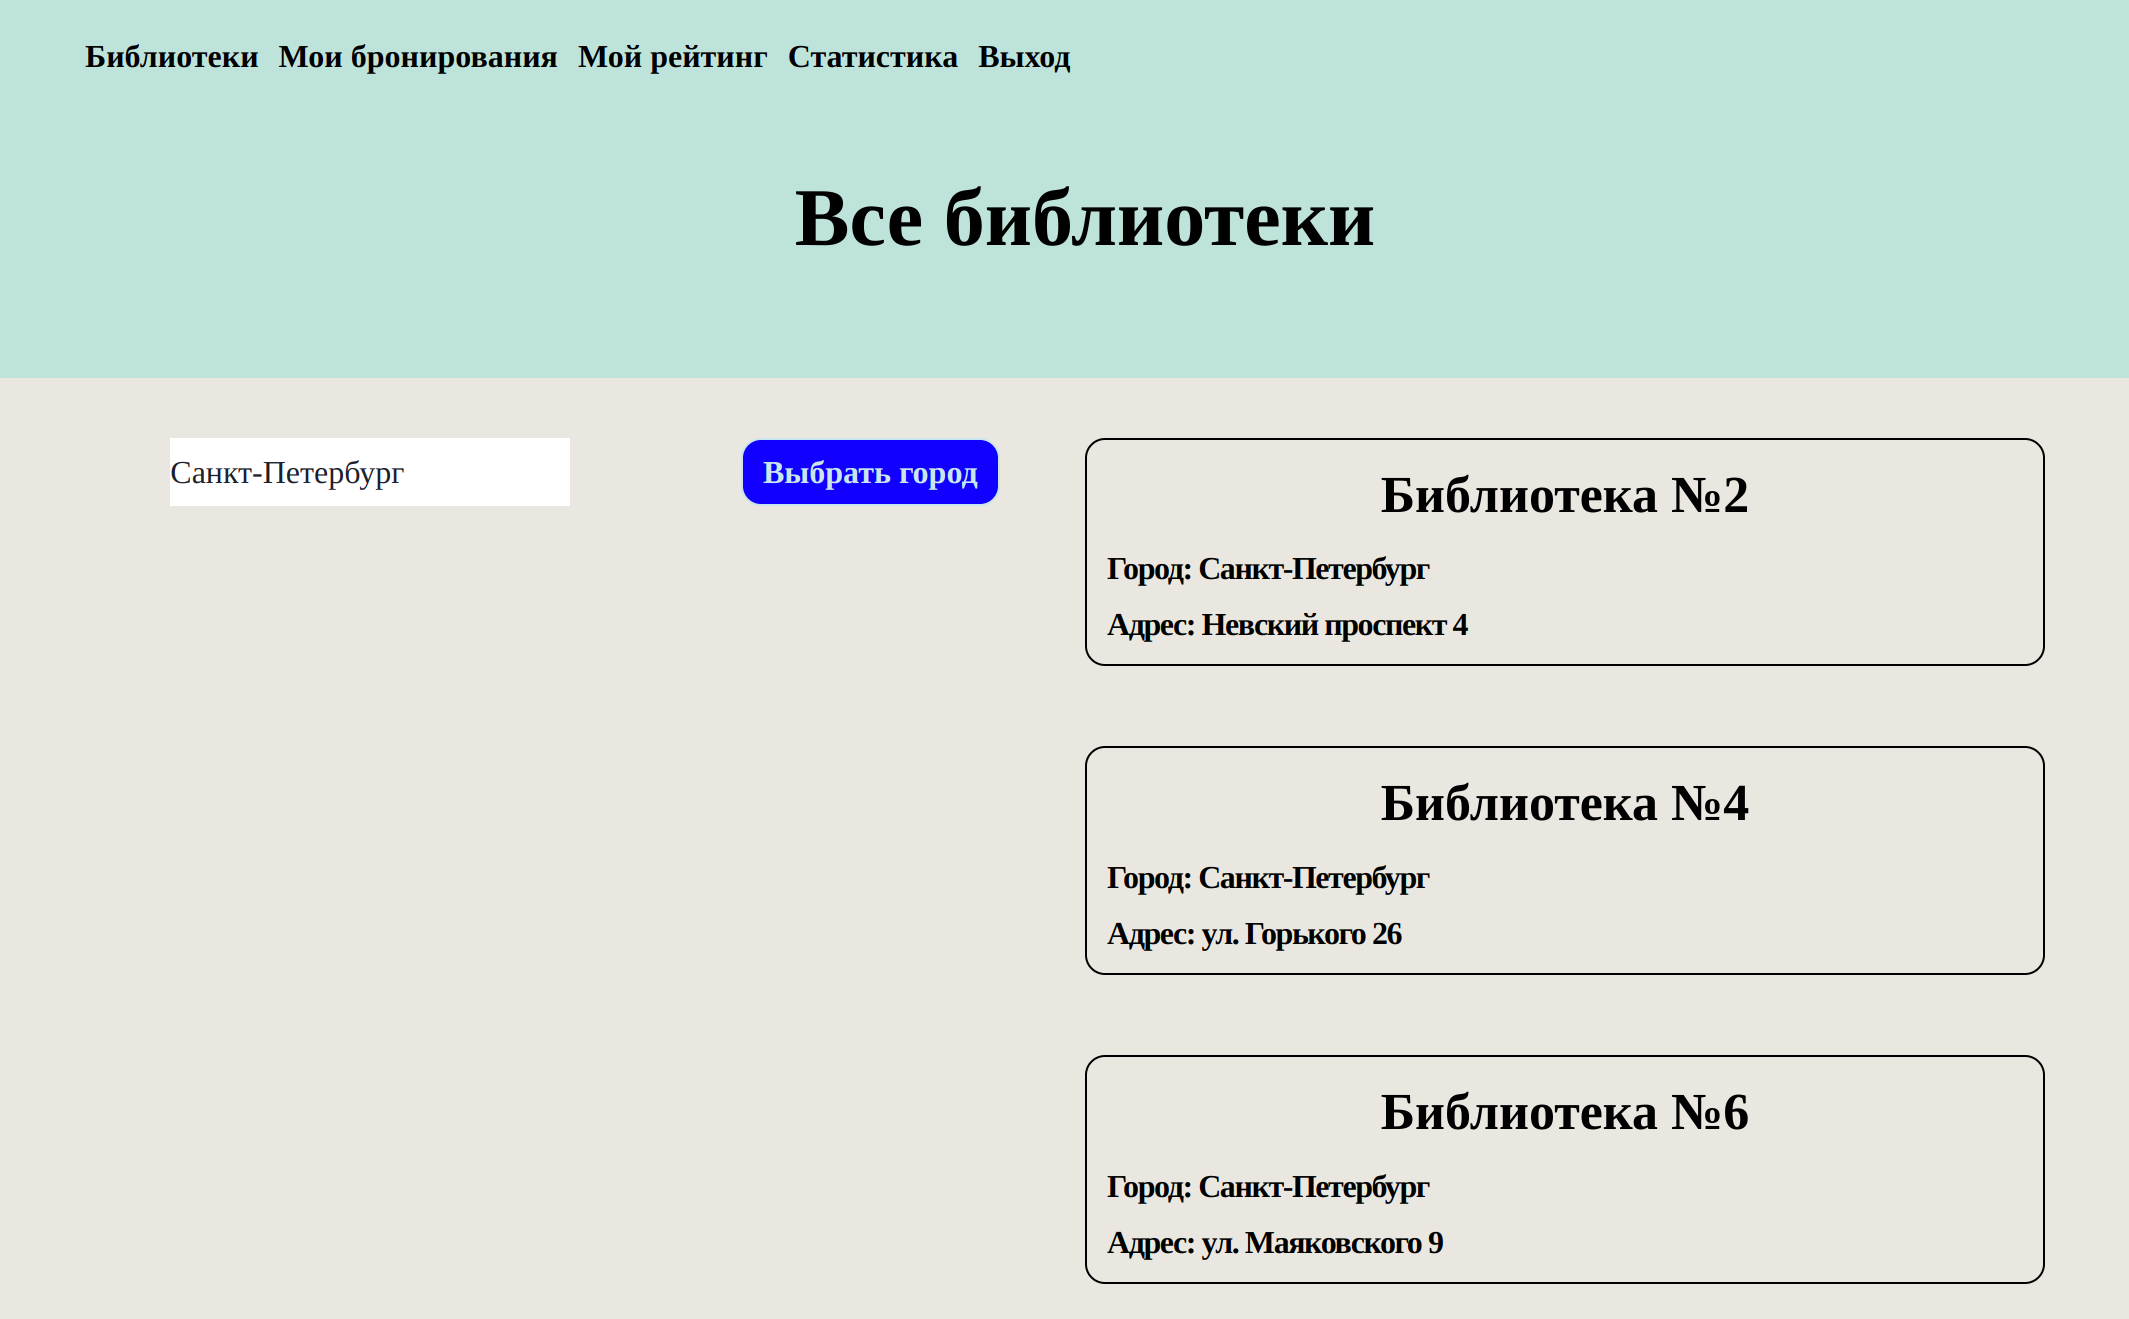
\includegraphics[scale = 0.2]{interface}}
		\caption{Интерфейс приложения}
		\label{fig:interface}
	\end{center}
\end{figure}

В приложении реализована деградация функциональности.
Например, в тестовых данных были бронирования, для которых указана несуществующая библиотека. 
При запросе дополнительной информации о библиотеке в сервисе библиотек срабатывало исключение и возвращалась 500 ошибка.
При этом страница отобразилась корректно, остались лишь пропуски на месте несуществующей библиотеки, как показано на рисунке \ref{fig:degradation}. 


Также была реализована ролевая модель.
Роль пользователей считывается сервисами из JWT-токена и выполняется проверка соответствия роли пользователя той роли, которой разрешен запрос.
Например, сервис статистики доступен только администратору.
Клиент при запросе статистики увидит сообщение, приведенное на рисунке \ref{fig:roles}. 

\newpage
\begin{figure}[h!]
	\begin{center}
		{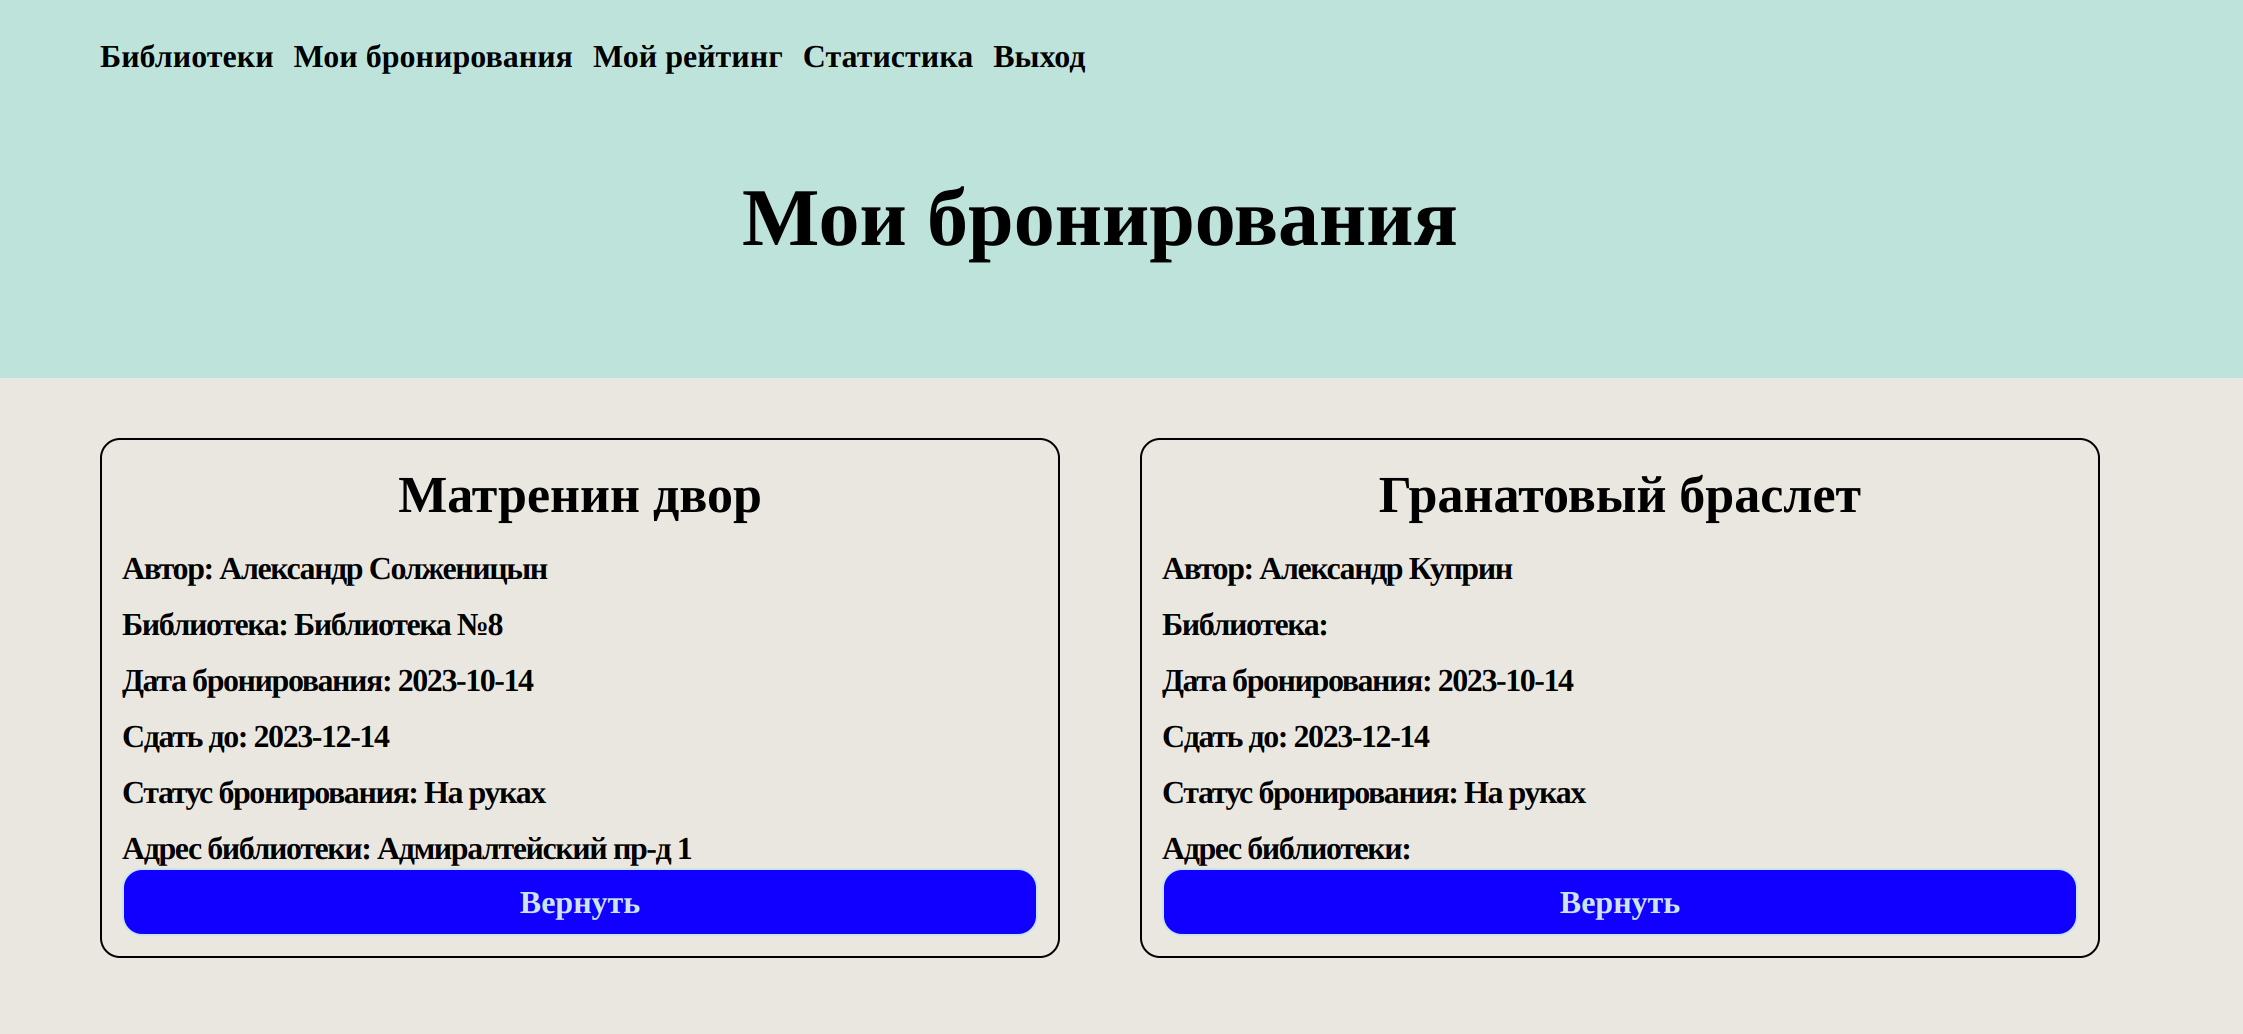
\includegraphics[scale = 0.2]{degradation}}
		\caption{Деградация функциональности при ошибке в сервисе библиотек}
		\label{fig:degradation}
	\end{center}
\end{figure}

\begin{figure}[h!]
	\begin{center}
		{
\includegraphics[scale = 0.2]{roles}}
		\caption{Сообщение о недостатке прав для обычного пользователя}
		\label{fig:roles}
	\end{center}
\end{figure}


\newpage
\titleformat{\section}[block]
{\bfseries\large\center}{\thesection}{1em}{}
\section*{ЗАКЛЮЧЕНИЕ}
\addcontentsline{toc}{section}{ЗАКЛЮЧЕНИЕ}
В результате выполнения курсовой работы: 
\begin{itemize}
    \item[---] сформулированы основные требования к системе и ее подсистемам;
    \item[---] описана архитектура системы в виде диаграмм в нотациях UML и IDEF0, а также указаны некоторые сценарии её функционирования;
    \item[---] разработано, развернуто и протестировано программное обеспечение, выполняющее основные заявленные требования и функциональность.
\end{itemize}

Таким образом, была разработана распределенная система для бронирования книг в библиотеках.

\newpage
\section*{СПИСОК ИСПОЛЬЗОВАННЫХ ИСТОЧНИКОВ}
\addcontentsline{toc}{section}{СПИСОК ИСПОЛЬЗОВАННЫХ ИСТОЧНИКОВ}
\begin{enumerate}
    \item Что такое REST API [Электронный ресурс]. Режим доступа: \url{https://ru.hexlet.io/blog/posts/chto-takoe-rest-api} (дата обращения: 27.04.2024).
    \item Circuit Breaker pattern --- Azure Architecture Center | Microsoft Learn [Электронный ресурс]. Режим доступа: \url{https://learn.microsoft.com/en-us/azure/architecture/patterns/circuit-breaker} (дата обращения: 17.08.2024).
    \item JSON Web Token Introduction --- jwt.io [Электронный ресурс]. Режим доступа: \url{https://jwt.io/introduction} (дата обращения: 17.08.2024).
    \item Kubernetes Documentation | Kubernetes [Электронный ресурс]. Режим доступа: \url{https://kubernetes.io/docs/home/} (дата обращения: 17.08.2024).
    \item Ingress Controllers | Kubernetes [Электронный ресурс]. Режим доступа: \url{https://kubernetes.io/docs/concepts/services-networking/ingress-controllers/} (дата обращения: 17.08.2024).
    \item Helm | Docs [Электронный ресурс]. Режим доступа: \url{https://helm.sh/docs/} (дата обращения: 17.08.2024).
    \item Final: OpenID Connect Core 1.0 incorporating errata set 2 [Электронный ресурс]. Режим доступа: \url{https://openid.net/specs/openid-connect-core-1_0.html} (дата обращения: 21.08.2024).
    \item RFC 6749 --- The OAuth 2.0 Authorization Framework [Электронный ресурс]. Режим доступа: \url{https://datatracker.ietf.org/doc/html/rfc6749#section-1.3.1} (дата обращения: 21.08.2024).
    \item Apache Kafka [Электронный ресурс]. Режим доступа: \url{https://kafka.apache.org/documentation/} (дата обращения: 17.08.2024).
    \item PostgreSQL: Documentation [Электронный ресурс]. Режим доступа: \url{https://www.postgresql.org/docs/} (дата обращения: 20.06.2024).
    \item Documentation --- Keycloak [Электронный ресурс]. Режим доступа: \url{https://www.keycloak.org/documentation} (дата обращения: 20.08.2024).
    \item VK Cloud | Облачная ИТ-платформа бизнес-класса от VK [Электронный ресурс]. Режим доступа: \url{https://cloud.vk.com/} (дата обращения: 26.08.2024).
    \item Welcome! | minikube [Электронный ресурс]. Режим доступа: \url{https://minikube.sigs.k8s.io/docs/} (дата обращения: 26.08.2024).
\end{enumerate}

\end{large}
\end{document}